%--------- Tipo de documento y definicion de paquetes ----------
%---------------------------------------------------------------
\documentclass[11pt, letter, twoside]{book}
\usepackage[utf8]{inputenc}

\title{tesis}
\author{David Hernández Uriostegui}
%\date{February 2019}

\usepackage{graphicx,amssymb,amsmath,amsfonts,psfrag,fancyhdr,layout,appendix,subfig}
\usepackage[spanish]{babel}
%\usepackage[latin1]{inputenc}
\usepackage{makeidx}
\usepackage{fncychap}
\usepackage{caption}
\usepackage{enumitem}
\usepackage{array,tabularx}
\usepackage[T1]{fontenc}
\usepackage{booktabs}
\makeatletter
\newcommand\footnoteref[1]{\protected@xdef\@thefnmark{\ref{#1}}\@footnotemark}
\makeatother
%\usepackage[times]{quotchap}
\usepackage{epigraph}

%\usepackage{cite}
%\usepackage{subfigure}
\usepackage{float} %redefinicion de objetos flotantes
%\usepackage{ucs}
%\usepackage[utf8]{inputenc}


\usepackage[sort&compress]{natbib}

\usepackage{hyperref}
%\usepackage{tocbibind}

\usepackage{setspace} %Paquete para crear intelineados en cualquier parte del documento

%Para bibliogafía por capítulos con BibTeX
%\usepackage{natbib}%[sectionbib]{natbib} nonamebreak
%\usepackage[sort,nonamebreak,sectionbib,square]{natbib}
%\usepackage[sort&compress,comma,authoryear]{natbib}

%%%% Paquetes para bibliografía %%%%%%%
%\usepackage{natbib}
%\usepackage{babelbib}
%\usepackage[spanish, authoryear]{flexbib}
%\usepackage{chapterbib}

%This change labels of subfig

%\renewcommand{\thesubfigure}{\alph{subfigure}\arabic{subfiggroup}}
%\captionsetup[subfigure]{labelformat=simple,labelsep=colon,                    listofformat=subsimple}
%\captionsetup{lofdepth=2} This is in order to list the subfigures in the LOF

%This include theorem environments
\newtheorem{theorem}{Teorema}[chapter]
\newtheorem{lemma}[theorem]{Lemma}
\newtheorem{proposition}[theorem]{Proposition}
\newtheorem{corollary}[theorem]{Corolario}

%\newenvironment{proof}[1][Proof]{\begin{trivlist}
%\item[\hskip \labelsep {\bfseries #1}]}{\end{trivlist}}
\newenvironment{definition}[1]
{\par\noindent\textbf{Definición(#1)}\begin{itshape}\par\noindent}%
{\end{itshape}} 
%----------------------------------------
%\newenvironment{proof}[1][Proof]{\begin{trivlist}
%\item[\hskip \labelsep {\bfseries #1}]}{\end{trivlist}}
%\newenvironment{example}[1][Example]{\begin{trivlist}
%\item[\hskip \labelsep {\bfseries #1}]}{\end{trivlist}}
%\newenvironment{remark}[1][Remark]{\begin{trivlist}
%\item[\hskip \labelsep {\bfseries #1}]}{\end{trivlist}}

%\newcommand{\qed}{\nobreak \ifvmode \relax \else
%      \ifdim\lastskip<1.5em \hskip-\lastskip
%      \hskip1.5em plus0em minus0.5em \fi \nobreak
%      \vrule height0.75em width0.5em depth0.25em\fi}
%----------------------------------------

\makeatletter
 \renewcommand{\p@subfigure}{}
  %Esto lo agrego yo para tener subfiguras a1, b1, ... a2, b2, ... 
  %Se reinicia cada vez que una nueva figura es convocada (como es debido).
  \newcounter{subfiggroup}[figure] 
\makeatother

%\usepackage[spanish]{babel}
\usepackage{epsfig}
\usepackage{url}
%Esto genera enlaces en el PDF
%\usepackage{latex2html}
%Esto es para el conversor latex2html
\usepackage{color}
%Esto cambia la coma por el punto decimal en las cifras 
\spanishdecimal{.}
\pagecolor{white}

%Este mejora las prestaciones de "\verbatim"
\usepackage{verbatim}

%Definición de margenes
\usepackage[left=3.4cm,top=2.5cm,right=2.6cm,bottom=2.5cm]{geometry}
\sloppy
\pagestyle{empty}

% Code for creating empty pages
% No headers on empty pages before new chapter

\makeatletter
\def\cleardoublepage{\clearpage\if@twoside \ifodd\c@page\else
    \hbox{}
    \thispagestyle{plain}
    \newpage
    \if@twocolumn\hbox{}\newpage\fi\fi\fi}
\makeatother \clearpage{\pagestyle{plain}\cleardoublepage}

% Code for creating fully-empty pages
% Fully empty pages before command is called
\makeatletter
\def\clearfullypage{\clearpage\if@twoside \ifodd\c@page\else
    \hbox{}
    \thispagestyle{empty}
    \newpage
    \if@twocolumn\hbox{} \newpage\fi\fi\fi}
\makeatother \clearpage{\pagestyle{empty}\clearfullypage}

% Dutch style of paragraph formatting, i.e. no indents.
\setlength{\parskip}{1.3ex plus 0.2ex minus 0.2ex}
\setlength{\parindent}{15pt}  % longitud de la sangría
%Leyendas de las graficas en letra pequeña, negrita, margen 2.5 y sangradas...
\captionsetup{font=small, labelfont={bf}, margin=2.5cm, format=hang}

%\setlength{\captionmargin}{60pt} %Margen de los pies de figura

%\includeonly{edicion}
%\includeonly{jurado,apoyo,licencia,edicion,reconocimientos,tvs}

% Double space for REVISION
%\renewcommand{\baselinestretch}{2.0}

%Print subsubsection numbers and put them in TOC
\setcounter{secnumdepth}{3}
\setcounter{tocdepth}{3}

%-------- Fin tipo de documento y definicion de paquetes -------
%---------------------------------------------------------------


%--------------  Inicio del Documento Maestro ------------------
%---------------------------------------------------------------

\makeindex
%\renewcommand{\baselinestretch}{1.5}

\begin{document}
%Cambiar Cuadros por Tablas y lista de... Debe ir después de \begin{document}
\renewcommand{\listtablename}{Índice de tablas} 
\renewcommand{\tablename}{Tabla} 

%%%%%%%%%%%%%55%%%%%%%%%%%%%%%%%%%%%
\frontmatter

%---------------- Portada -------------------------------------
%% portada.tex-- Portada para tesis de posgrado de la Facultad de Ingeniería. UNAM.
% Realizada por Gengis Kanhg Toledo Ramírez (gengiskanhg.geo@yahoo.com)
%Basada en la portada escrita por: Tim Rohrer, LT, USN--31 July 1996 del NPS, Monterey, California. USA.
%y en el manual The Not So Short Introduction to LaTeX de Tobiaz Oetiker
%Eres libe de modificar este archivo de acuerdo a tus necesidades.
%13 de Junio de 2007

%Compile with:
%pdflatex portada.tex

\documentclass{book}

\usepackage[utf8]{inputenc}
%\usepackage[latin1]{inputenc}
\usepackage[spanish]{babel}
\usepackage{graphicx}

\setlength{\voffset}{-0.5cm}
\setlength{\hoffset}{0.7cm}
\setlength{\headsep}{0pt}
\setlength{\headheight}{0pt}
\setlength{\oddsidemargin}{-0.8in}
\setlength{\marginparwidth}{-0.5cm}
\setlength{\textwidth}{19.5cm}
\setlength{\footskip}{2pt}
\setlength{\topmargin}{0in}
\setlength{\textheight}{25cm}
\setlength{\fboxrule}{3pt}

\begin{document}
\thispagestyle{empty}

\begin{tabular}{p{3cm}p{15.0cm}}
\includegraphics[width=3.3cm]{figuras/escudoUNAMbn.png}
%\includegraphics[natwidth=50bp,natheight=50bp, width=50bp]{figuras/escudoUNAMbn.png}
\begin{center}
\rule[0cm]{1.5mm}{18.5cm}%vertical
\hspace{2pt}
\rule[0cm]{0.5mm}{18.5cm}%vertical
\hspace{2pt}
\rule[0cm]{1.5mm}{18.5cm}%vertical
\end{center}
%\includegraphics[width=2.8cm]{figuras/escudoFI-UNAM.png}
&
\vspace{-3.4cm}
\begin{center}
\Large{ \bf{UNIVERSIDAD NACIONAL AUTÓNOMA DE MÉXICO}}
\\
\rule[0mm]{15.0cm}{0.2mm}%horizontal
\\
\rule[3mm]{15.0cm}{1.2mm}%horizontal
\\
\textsc{Posgrado en Ciencia e Ingeniería de la Computación}

%\vspace{1.0\baselineskip}

%INSTITUTO DE INVESTIGACIÓN EN \\ MATEMÁTICAS APLICADAS Y EN SISTEMAS

\vspace{3.5\baselineskip}

{\Large \bf{Título de la tesis}}

%\vfill
\vspace*{2.0cm}

\huge{\bf T  E  S  I  S}

\vspace*{0.2cm}
{\large QUE PARA OBTENER EL GRADO DE:}

\vspace*{1cm}

\Large{\bf MAESTRO EN CIENCIAS DE LA COMPUTACIÓN}

%\vspace*{0.2cm}
%\large{COMPUTACIÓN}

\vspace*{2.0cm}
{\large P R E S E N T A:}

\vspace*{0.5cm} {\Large \bf{NOMBRE DEL ALUMNO}}

\vspace*{2.0cm}
\large{DIRECTOR DE TESIS:}

\large{\bf DRA. HELENA M. GÓMEZ ADORNO}

\vspace*{2.5cm}
\large{C.U., Ciudad de México}\hspace*{7.2cm}\large{2019}

\end{center}

\end{tabular}

%\flushright{$^{*}$Exbecario CONACYT\hspace*{0.8cm}}

%\end{center}
%\newpage
%\thispagestyle{empty}
$ $
\end{document}

%Se compila aparte y se junta con "gs".
%gs -dNOPAUSE -sDEVICE=pdfwrite -sOUTPUTFILE=tesiscompleta.pdf -dBATCH portada.pdf tesis.pdf
%---------------------------------------------------------------


%------------------ Información preeliminar --------------------
%---------------------------------------------------------------

\singlespacing %Interlineado sencillo \usepackage{setspace}
\pagestyle{empty}
%\newpage
\vspace{0.5cm}
\Large{{\scshape Jurado asignado:}}

\vspace{2.0cm}
\begin{tabular}{l l}
\Large{Presidente:} & \Large{Dr... } \\
\\ 
\Large{Vocal:} & \Large{Dra....}\\
\\
\Large{Secretario:} & \Large{Dr....}\\
\\
\Large{Suplente:} & \Large{Dra....}\\
\\
\Large{Suplente:} & \Large{Dr....}\\
\\ 
\end{tabular}

\vspace{2.5cm}

\begin{center}
\Large{ \scshape{Directora de tesis:}}
\vspace{0.8cm}

% Espacio para dos tutores cambiado para uno solamente
%\begin{tabular}{c p{0.5cm} c}
%\rule[0mm]{5.0cm}{0.2mm} & &\rule[0mm]{5.0cm}{0.2mm} \\
%\Large{\bf Dr. Ernst Kussul.} & &\Large{\bf Dra. Tatiana Baidyk.} \\ 
%\end{tabular}

\rule[0mm]{6.5cm}{0.2mm} \\
\Large{\bf Dra. Helena M. Gómez Adorno} \\


\end{center}
\normalsize

%%% Local Variables: 
%%% mode: latex
%%% TeX-master: "tesis"
%%% End: 

%\clearfullypage
%\pagenumbering{roman}
%Página de quienes dieron apoyo

%\newpage
%\begin{flushright}
\vspace*{16.5cm}

\begin{tabular*}{\textwidth}{p{4cm} p{10cm}}

\\
\end{tabular*}

%\end{flushright}


%%% Local Variables: 
%%% mode: latex
%%% TeX-master: "tesis"
%%% End: 

%Página de licencia

\newpage
%\begin{flushleft}
\vspace*{19cm}
\begin{tabular*}{\textwidth}{p{10cm} p{5cm}}
El autor, sin perjuicio de la legislación de la Universidad Nacional Autónoma de México, otorga el permiso para el libre uso, reproducción y distribución de esta obra siempre que sea sin fines de lucro, se den los créditos correspondientes y no sea modificada en ningún aspecto.&  \\
& \\
D.R. \copyright Nombre del Alumno \hspace{1cm} México D.F., 2019. & \\
\end{tabular*}

%\end{flushleft}

%%% Local Variables: 
%%% mode: latex
%%% TeX-master: "tesis"
%%% End: 

%\clearfullypage
%Página de dedicatoria

\newpage
%\begin{flushright}
\vspace*{6cm}

\begin{center}

%\hspace{0.4cm}


Dedicatorias....

\vspace{0.5cm}
\vspace{1cm}


\end{center}

%\end{flushright}


%%% Local Variables: 
%%% mode: latex
%%% TeX-master: "tesis"
%%% End: 




%\include{frases}
%\clearfullypage

\chapter*{Agradecimientos}
\epigraph{``Un individuo solo, sólo no puede transcender.''
}{\textit{Carlos Salinas de Gortari}}
\noindent 

\noindent

\begin{flushright}
\textit{Ciudad Universitaria, IIMAS, 2019}
\end{flushright}
 



%%% Local Variables: 
%%% mode: latex
%%% TeX-master: "tesis"
%%% End: 


%\color[rgb]{0,0,0}

% Define pagestyle
\pagestyle{fancy}
\fancyhf{}
\renewcommand{\chaptermark}[1]{\markboth{ \emph{#1}}{}}
\fancyhead[LO]{}
\fancyhead[LO]{}
\fancyfoot[LE,RO]{\thepage}

% Redefine plain page style
%---------------------------------
\fancypagestyle{plain}{
\fancyhf{}
\renewcommand{\headrulewidth}{0pt}
\fancyfoot[LE,RO]{\thepage}
}
%---------------------------------

% Dutch style of paragraph formatting, i.e. no indents.
\setlength{\parskip}{1.3ex plus 0.2ex minus 0.2ex}

% Remove parskip for toc
\setlength{\parskip}{0ex plus 0.5ex minus 0.2ex}

\tableofcontents
\listoffigures
\listoftables

%\cleardoublepage
%\clearfullypage
\addcontentsline{toc}{chapter}{Resumen}

\begin{center}
\large{\bf Desarrollo de un Tablero de Datos para un Sistema de Información Hospitalaria}

\normalsize{Tesis de Licenciatura}\\
\vspace{0.5cm}

\normalsize{\bf David Hernández Uriostegui\\
Licenciatura en Ciencias de la Computación}\\
Universidad Nacional Autónoma de México

\vspace{1.0cm}

\large{\textbf{Resumen\\}}

\end{center}
La Secretaría de Salud de la Ciudad de México (SEDESA) tiene implementada desde el 2014 la plataforma del Sistema de Administración Médica e Información Hospitalaria (SAMIH), catalogada como una de las mejores al cumplir con el protocolo \text{HL7} (Health Level Seven), en 30 Hospitales de la red hospitalaria institucional. Este sistema de información apoya las actividades en los niveles operativo, táctico y estratégico en los hospitales. Para ello utiliza sistemas que permiten recabar, almacenar y procesar información clínica y administrativa, y los expedientes clínicos de cada uno de los usuarios atendidos, que contienen información relevante para los profesionales de la salud y la historia médica del paciente, sus antecedentes, diagnósticos y pronósticos en salud (Morales-Velázquez, 2019). Mediante SAMIH el sistema de salud de la Ciudad de México puede disponer de información y generar datos de salud útiles para mejorar la gestión médico-administrativa y facilitar la toma de decisiones. Sin embargo, el propósito del SAMIH busca otros fines y para atender necesidades de información como lo fue requerido durante la pandemia del COVID-19 es necesario robustecer ciertas funcionalidades y aumentar otras.\\

Una de las principales necesidades de la SEDESA ante la contingencia sanitaria fue el contar con información de calidad y oportuna, que permita la óptima administración de los recursos en salud y garantizar el derecho efectivo a la salud de la población de la Ciudad de México. Motivo por el cual, urge superar algunas de las limitantes actuales para lograr, en un corto plazo, hacer frente a la pandemia de COVID-19 y, en un mayor plazo, lograr establecer un sistema de información en salud resiliente ante contingencias futuras.\\

Este proyecto busca que la SEDESA y el Gobierno de la Ciudad de México puedan acceder a información contenida en SAMIH mediante un tablero analítico con información estadística de los pacientes que se encuentran hospitalizados. El sistema propuesto permitirá robustecer las funcionalidades de sistema de información hospitalaria de la SEDESA, facilitar la administración de los recursos en salud, mejorar la atención hospitalaria de los pacientes y, en última instancia, contribuir a garantizar el derecho efectivo a la salud de la población de la Ciudad de México (Ayaad et al., 2019).\\

Se publicarán los resultados obtenidos del modelo del tablero analítico y los resultados de la extracción de información de los expedientes clínicos a partir de técnicas de procesamiento de lenguaje natural, contribuyendo a la generación de conocimiento científico y la formación de recursos humanos. Además, el sistema permitirá la extracción sistemática de información relevante de los pacientes hospitalizados para fines de investigación, cuyos resultados, a la vez, contribuirán a la toma de decisiones.
 
%%% Local Variables: 
%%% mode: latex
%%% TeX-master: "tesis"
%%% End: 
 
%\cleardoublepage
%Resumen en inglés
\addcontentsline{toc}{chapter}{Summary}

\begin{center}
\large{\bf Title}

\normalsize{MSc Thesis}\\
\vspace{0.5cm}

\normalsize{\bf Nombre Alumno}\\
Posgrado en Ciencia e Ingeniería de la Computación\\
Universidad Nacional Autónoma de México

\vspace{1.0cm}

\large{\textbf{Summary\\}}

\end{center}
Lorem ipsum dolor sit amet, consectetur adipiscing elit. Vestibulum viverra porta diam, quis placerat leo blandit sit amet. Nam enim sem, pellentesque vel mi quis, condimentum mattis lectus. Cras in sapien suscipit, ullamcorper turpis eget, venenatis quam. Maecenas non ipsum auctor nisi venenatis volutpat sit amet at lorem. Donec at dignissim eros, vitae maximus mauris. Nullam et orci mattis, volutpat nisi nec, condimentum leo. Morbi scelerisque tristique imperdiet.

Lorem ipsum dolor sit amet, consectetur adipiscing elit. Quisque interdum dolor non aliquet rutrum. Duis congue mauris ut urna rutrum, in vulputate metus volutpat. Phasellus dui dui, laoreet nec purus eu, auctor feugiat libero. Aliquam placerat tellus lacinia, pulvinar lorem ac, faucibus justo. Morbi interdum odio ligula, sed mattis nisi pulvinar nec. Aenean dapibus imperdiet nulla placerat tristique. Maecenas consectetur dui a nibh ullamcorper sollicitudin. Integer vestibulum ante quis metus vestibulum, sollicitudin auctor est blandit. Morbi bibendum ultricies dignissim. Maecenas sodales risus ut purus congue blandit. Proin pretium augue et dignissim vulputate.

Morbi nulla nunc, feugiat fermentum nisl vitae, sollicitudin tincidunt leo. Duis bibendum ipsum justo, lacinia sodales lorem rutrum et. In mattis varius tortor, id placerat erat imperdiet a. Curabitur convallis dui non posuere facilisis. Aenean varius mauris eu semper viverra. Nulla semper eget sem at malesuada. Integer porta varius ligula non egestas. Donec dignissim quam sit amet felis tincidunt, vel scelerisque elit placerat. Integer ornare felis et sem euismod suscipit. Curabitur a nisi ac metus ultricies laoreet in at nunc. Maecenas auctor libero sit amet rutrum consectetur. Pellentesque sit amet accumsan metus, venenatis vulputate erat. Cras egestas vel turpis vitae dapibus.

%%% Local Variables: 
%%% mode: latex
%%% TeX-master: "tesis"
%%% End: 
 
%\cleardoublepage


%------------------- Fin información preeliminar----------------
%---------------------------------------------------------------


%------------------- Capítulos de la tesis ---------------------
%---------------------------------------------------------------


% Adjustments headers
\fancyhead[RO]{\leftmark}

%%%%%%%%%%%%%
\mainmatter
%%%%%%%%%%%%%
\pagenumbering{arabic}
% Adjustments headers
\fancyhead[RO]{\leftmark}
\fancyhead[EL]{\emph{Capítulo \thechapter}}
%\setcounter{page}{3}

\medskip
%Interlineados  \usepackage{setspace}
%\onehalfspacing 
\singlespacing
%Introduccion
\chapter{\bf{Introducción}}\label{cap:intro}
%\epigraph{``Frase opcional''
%}{\textit{Autor}}

%Como capitulo introductorio, se explicará y abordará de manera general la problemática que desembocó la motivación del trabajo, así como los objetivos a realizar para la implementación del proyecto, ejemplos de tecnologías desarrolladas durante la pandemia de COVID-19 para ayudar a llevar un control sobre los contagios.

En este primer capítulo introductorio, se abordará de manera general la problemática que motivó la realización de este trabajo. Se explorará el contexto que llevó a la necesidad de mejorar los procesos de almacenamiento y análisis de datos en la Secretaría de Salud de la Ciudad de México (\textbf{SEDESA}).

Además, se hablará de los objetivos  que orientan la implementación de este proyecto. Se proporcionarán ejemplos de tecnologías desarrolladas durante la pandemia de COVID-19 que han demostrado ser eficaces para el control de contagios y que sirven como referencia para el enfoque adoptado en este proyecto.


\section{Planteamiento del Problema}\label{intro_mot}
%Escribir que motivó el trabajo de investigación....
%Cual es el problema que queremos abordar: En este caso sería el desarrollo de un tablero de datos con información agregada de pacientes.... aqui se puede mencionar las tecnologías que se van a utilizar para para el desarrollo. Hablar sobre la importancia de utilizar software open source debido a la falta de recursos para licencia por parte de la Secretaria de Salud (aqui también puedes mencionar que los recursos económicos durante tiempo de pandemia fue necesario utilizar el materiales, salarios de los médicos, etc.)

La creación de una aplicación web destinada a la gestión de información hospitalaria por parte de la Secretaría de Salud de la Ciudad de México (\textbf{SEDESA}) surge como respuesta a la necesidad de mejorar los procesos de almacenamiento y análisis de datos para esta institución. La complejidad y volumen de la información manejada por la \textbf{SEDESA} demandan una herramienta eficiente que permite al personal la gestión interna de pacientes y seguimiento de métricas dentro de los hospitales \cite{morales2019sistema}.

El objetivo principal durante el proyecto, fue el desarrollo de un tablero de datos diseñado específicamente para proporcionar información clave sobre pacientes que habían contraído \textsc{COVID-19}.
En dicho tablero se presentan diversas métricas relacionadas con el manejo de pacientes afectados por \textsc{COVID-19}, incluyendo datos sobre ingresos y egresos hospitalarios, defunciones causadas por la enfermedad y traslados entre diferentes centros de atención médica.

Para llevar a cabo el modulo del tablero de datos, se utilizaron tecnologías para la implementación de aplicaciones web que se encuentran entre las más utilizadas en la actualidad en el mercado como lo son \texttt{React} y \texttt{Django}, el usarlas no sólo garantiza la eficiencia y la fiabilidad del sistema, sino que también permite la adaptabilidad continua a medida que se lanzan nuevas versiones.

La elección de utilizar software \textit{Open Source} \footnote{El software \textit{Open Source} es un software que se distribuye con su código fuente, lo que permite su uso, modificación y distribución con sus derechos originales.} fue fundamental en el desarrollo de esta aplicación, dada la situación económica y la prioridad de asignar recursos a áreas de mayor importancia por parte \textbf{SEDESA}, como el material médico, salarios del personal sanitario y otros aspectos esenciales durante la crisis sanitaria del \textsc{COVID-19}.

De igual manera, esta decisión a corto, mediano y largo plazo permitirá la colaboración en el desarrollo tecnológico. El nuevo personal que contribuya al desarrollo puede mejorar constantemente la aplicación, lo cual permite así una evolución continua y adaptación a las necesidades cambiantes de la Secretaría de Salud.

\section{Objetivos}\label{intro_obj}
El objetivo general de este trabajo consiste en el desarrollo de un módulo de la aplicación web dónde se muestre un tablero con diferentes gráficas que presentan métricas relacionadas a pacientes hospitalizados que estuvieron contagiados de \textsc{COVID-19}.

Como en toda aplicación web, esta se compone por 2 partes: \textbf{Frontend} y \textbf{Backend}.

Por lo tanto, podemos descomponer los objetivos en los que conciernen al \textbf{Frontend} y los relacionados al \textbf{Backend}.

\begin{itemize}
    \item \texttt{Backend}
        \begin{itemize}
            \item Desarrollo de endpoints para obtener los datos necesarios para los componentes de visualización del \textbf{Frontend}.
            \item El diseño y la implementación de consultas SQL que cumplen con los requisitos de información especificados.
        \end{itemize}
    \item \texttt{Frontend}
        \begin{itemize}
            \item Creación de componentes en \texttt{ReactJS} para la visualización de las gráficas.

            \item Llamada a endpoints creados en el backend para la obtención de los datos para los módulos de visualización.
        \end{itemize}
    
\end{itemize}

\section{Antecedentes}\label{hipótesis}
%Durante la pandemia, se comenzó a requerir y desarrollar herramientas eficientes para recopilar, procesar y analizar datos relacionados con la salud pública. 


El surgimiento de la enfermedad \textsc{COVID-19}, causada por el virus \textsc{SARS-CoV-2}, ha representado un episodio de gran trascendencia en los últimos años al desencadenar una crisis de alcance global. Su propagación rápida, gran capacidad de mutación y la diversidad de manifestaciones clínicas, que van desde síntomas leves hasta casos graves, han desafiado a las comunidades globales y resaltado la necesidad de respuestas conjuntas a nivel internacional.

La mayoría de los países han aplicado cierres y medidas sanitarias para evitar su propagación. Sin embargo, a pesar de que estas medidas han funcionado de una manera racional, un bloqueo prolongado es insostenible. Por ello, la opinión generalizada es que las pruebas y el rastreo de virus son un gran apoyo para facilitar las medidas de bloqueo.

Hoy en día, se han desarrollado diversas aplicaciones y software para poder realizar análisis de datos sobre el impacto de la pandemia en diferentes ámbitos, como el sistema sanitario, los sistemas de transporte, el sistema educativo, la prestación de servicios gubernamentales, las empresas farmacéuticas, la fabricación, las industrias de software y las empresas multinacionales \cite{ayaad2019role} \cite{delrosario2021procesamiento}.

El volumen de datos que se ha generado en todos los ámbitos anteriormente mencionado es de gran tamaño, estos son generados principalmente fuentes, como la Organización Mundial de la Salud (\textbf{OMS}), redes sociales, hospitales públicos y privados, pacientes e instituciones académicas, que necesitan un mecanismo eficaz de análisis de datos para gestionar estos datos de forma eficiente. Lo cual ha conllevado al desarrollo de mecanismos que permitan realizar un manejo de datos a baja, mediana y gran escala, dependiendo de las necesidades de la entidad que haya pedido el desarrollo del sistema \cite{fan2023accessibility}.

Por ejemplo, \textbf{DHIS2} \footnote{Link donde se puede consultar \textbf{DHIS2}: https://dhis2.org/covid-19/} es un aplicación web para la recopilación, gestión y análisis de datos relacionados a la salud. En cuanto a su uso que concierne al \textsc{COVID-19}, incluye herramientas para la aceleración de la detección de casos, la información sobre las medidas de respuesta y la supervisión de la distribución equitativa de las vacunas. En la actualidad, \textsc{DHIS2} es la mayor plataforma de sistemas de gestión de la información sanitaria del mundo, utilizada por ministerios de sanidad de 80 países.

De igual manera, existen diversas aplicaciones y tableros como en la que se trabajó, las cuales son para manejo de datos más privados o un volumen de datos menos pesado. Un ejemplo a gran escala, son los tableros de datos implementados por el Mtro. Manuel Antonio Mojica Baltodano en Power BI por que muestran el impacto del COVID-19 tanto en América Latina como en el resto del mundo \cite{mojica2020tableros}. De igual manera, existen tableros enfocados en zonas más especificas como el tablero de datos desarrollado por investigadores de la Pontificia Universidad Católica de Chile, enfocado en la población atendida en los establecimientos de salud de Atención Primaria de la Corporación Municipal de Viña del Mar, entre los años 2021 y 2022~\cite{gomez2023analisis}.

En conclusión, el \textsc{COVID-19} ha puesto de manifiesto la importancia de contar con herramientas tecnológicas robustas y flexibles para analizar y gestionar datos en diferentes escalas y contextos. La diversidad de aplicaciones, desde plataformas a gran escala como \textsc{DHIS2} hasta soluciones más específicas, indica la necesidad de adaptarse a la complejidad de la información generada durante crisis sanitarias.

\section{Contribución}\label{intro_cont}
Las contribuciones de este trabajo se enfocaron en el proceso de desarrollo de un tablero de datos especializado para la gestión de pacientes con \textsc{COVID-19}, construido a partir de un \textit{mockup} \footnote{Un \textit{mockup} es una visualización o diseño de una aplicación, página web o producto que ilustra el aspecto que podría tener el resultado final.} proporcionado por \textsc{SEDESA}. 

\begin{enumerate}
    \item \textbf{Transformación de \textit{Mockup} a Realidad:} Se está llevando a cabo la traducción del \textit{mockup} proporcionado. Este proceso forma parte del \textit{frontend} y actualmente se está trabajando en la parte visual del tablero. Utilizando la tecnología \texttt{ReactJS}, se están implementando componentes interactivos que se espera reflejen con precisión la estructura y el diseño del \textit{mockup}.

    
    \item \textbf{Integración con el \textit{Backend}:} Se desarrollaron \textit{endpoints} específicos en el \textit{backend} para obtener los datos necesarios para los componentes de visualización en el \textit{frontend}. Esta integración en desarrollo busca garantizar la obtención eficiente de datos, permitiendo que el tablero se mantenga actualizado y refleje con precisión la información más reciente sobre pacientes y métricas asociadas.
    
    \item \textbf{Flexibilidad para Mejoras Continuas:} La implementación en desarrollo, al estar basada en tecnologías \textit{Open Source}, busca proporcionar no solo para las necesidades actuales, sino también una base sólida para futuras mejoras y adaptaciones.
\end{enumerate}

En resumen, la contribución principal de este proyecto está enfocada en el proceso de desarrollo de un tablero de datos basado en un \textit{mockup} previamente proporcionado, con la finalidad de proporcionar una herramienta para la gestión de información hospitalaria de \textbf{SEDESA} relacionada con pacientes afectados por COVID-19.

%{\large \bf{Logros}}\\
%\section{Logros}
%\label{intro_log}
%\index{logros}

%Desarrollar un modelo que aplique las técnicas de transferencia de conocimiento a la tarea de perfilado de autor

%{\large \bf{Organización de  perla Tesis}}\ \
\section {Organización del documento}\label{intro_org}
%\index{organización}

A continuación se describen los capítulos que componen este documento:

\begin{enumerate}
    \item \textbf{Marco Teórico}\\
    En este capítulo se describen conceptos y términos que se utilizarán en el desarrollo de este proyecto como lo son \texttt{PostegreSQL, Django} y \texttt{ReactJS}.

    \item \textbf{Estado del arte}\\
    En este capitulo se menciona que se está utilizando hoy en día en la industria para implementar tableros de datos. También, se habla del software \textit{Open Source} y de paga, así como un comparación entre ellos. 

    \item \textbf{Metodología propuesta}\\
    En este capítulo se describe el marco metodológico de este trabajo de investigación, cómo funciona la conexión entra la base de datos, el \textit{backend} y \textit{frontend}.

    \item \textbf{Construcción final del tablero de información de pacientes COVID-19}\\
    En este capítulo se explica a detalle como funciona el tablero, se describen los parámetros que recibe para el despliegue de las gráficas en cada una de las secciones.
    
    \item \textbf{Conclusiones y trabajo futuro}\\
    En éste capítulo se presentan las conclusiones finales del presente trabajo de tesis y el trabajo que se planea y que se podría implementar a futuro.

\end{enumerate}


%Perfilado de autor
\setlength{\arrayrulewidth}{0.5mm}
\setlength{\tabcolsep}{18pt}
\renewcommand{\arraystretch}{1.5}


\chapter{Marco Teórico} \label{cap:antecedentes}




Este capitulo se dedica a explorar y contextualizar los conceptos, tecnologías y metodologías esenciales que fundamentan la implementación del tablero de datos propuesto. 

En este contexto, se abordarán conceptos clave como \texttt{PostgreSQL}, \texttt{Django}, y \texttt{ReactJS}, que desempeñan un papel fundamental en el diseño y funcionamiento de la aplicación. Además, hará una comparativa en diferentes bibliotecas y software para la visualización de datos, y el por qué se eligió el uso de la biblioteca \texttt{AmCharts} para la implementación del tablero.

El enfoque de este capítulo es proporcionar una comprensión  de las herramientas y tecnologías seleccionadas para el desarrollo del tablero de datos. Se profundizará en sus características, ventajas y casos de uso relevantes, estableciendo así una base sólida para la posterior discusión de la metodología y la construcción del tablero de datos.

\section{Base de datos}\label{sec:basedatos}
Las bases de datos son componentes esenciales en el ámbito de las ciencias de la computación y más en especifico, en la creación de software. Proporcionan un mecanismo estructurado y eficiente para almacenar, organizar y recuperar datos de manera sistemática. 

Más en concreto, en lo que concierne a las aplicaciones web, el uso de bases de datos permite gestionar grandes volúmenes de información de manera estructurada y accesible.

Existen diferentes tipos de bases de datos, y la elección del tipo adecuado depende de los requisitos específicos de la aplicación. 

\subsection{Modelo relacional}
Hoy en día, el modelo de bases de datos más usado en todos los ámbitos, es el \textbf{relacional}. Este modelo se basa en la representación de datos en tablas, proporcionando una forma clara y estructurada de organizar la información. Cada tabla contiene registros que representan entidades únicas y columnas que almacenan atributos específicos de esos registros. La relación entre tablas se establece mediante claves únicas, permitiendo la conexión y consulta eficiente de datos.

%\textcolor{red}{La Figura \ref{fig:ejemploRelacional} está aislada, no tiene ninguna descripción que indique al lector que es lo que se quiere mostrar con esta gráfica. Todas las figuras que agregues al documento deben estan referenciadas y explicadas.}

\begin{figure}[!h]
\centering
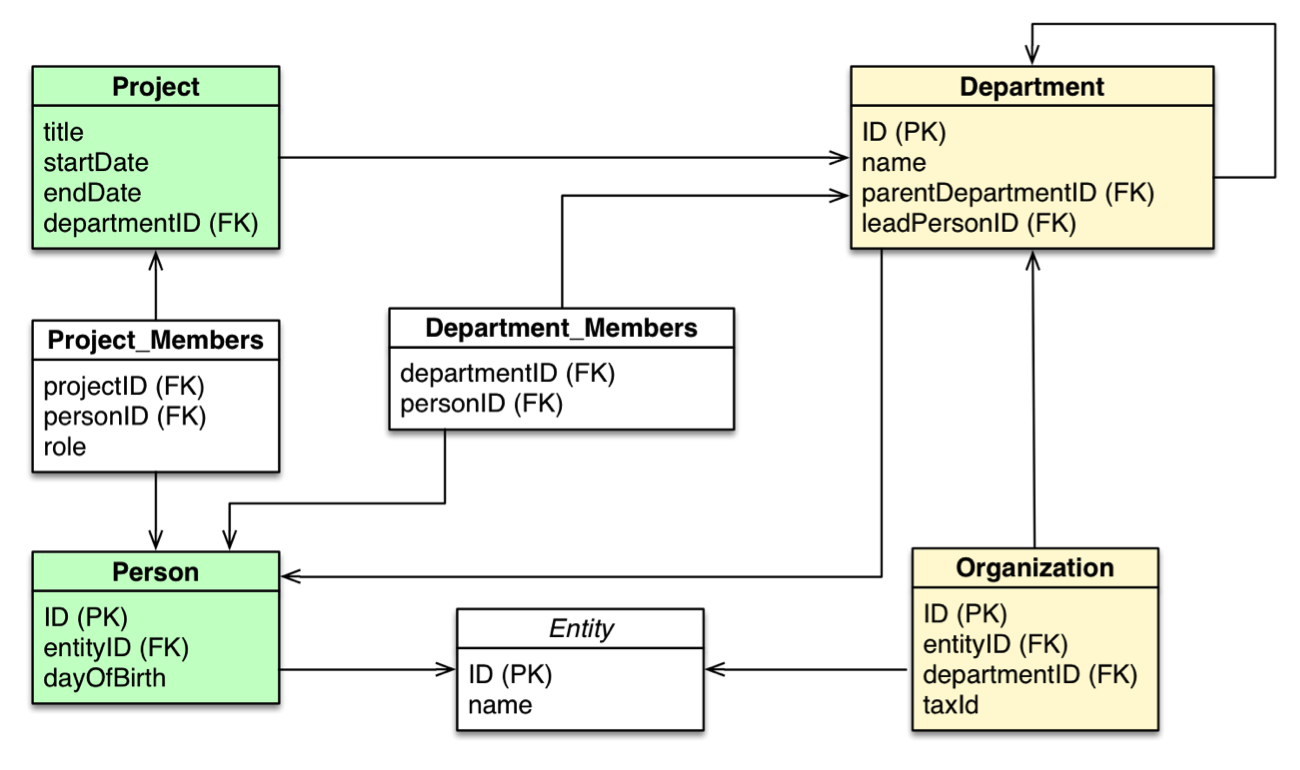
\includegraphics[width=0.5\textwidth]{images/ejemplo-modelo-relacional.png}
\caption{Modelo relacional representando una empresa con tablas interconectadas}\label{fig:ejemploRelacional}
\end{figure}

Las bases de datos relacionales se basan en el modelo relacional, ya que este proporciona una forma estructurada de representar datos en tablas. En una base de datos relacional, cada fila de la tabla es un registro con un \textbf{\texttt{ID}} único denominado clave. Las columnas de la tabla contienen atributos de los datos, y cada registro suele tener un valor para cada atributo, lo que facilita establecer las relaciones entre los puntos de datos~\cite{sql_thesis1}. 
Un ejemplo ilustrativo se presenta en la Figura \ref{fig:ejemploRelacional}, donde se muestra un modelo relacional que representa una empresa, el cual contiene varias tablas que están interconectadas a través de columnas que establecen relaciones entre ellas.


\subsection{Sistema de gestión de bases de datos}

Teniendo definido un modelo para implementar una base de datos, se debe tener un medio o herramienta con la cual interactuar para realizar operaciones como crear y borrar tablas, insertar y borrar datos, dar permisos de lectura y/o alteración, entre otro tipo de operaciones.

Para ejecutar este tipo de operaciones se utilizan los 
\textit{Sistema de gestión de bases de datos}. 

Un \textbf{Sistema de gestión de bases de datos \textit{(DBMS, Data Base Management System)}} es un software que sirve como interfaz entre la base de datos y sus programas o usuarios finales, lo que permite a los usuarios recuperar, actualizar y gestionar cómo se organiza y se optimiza la información. Un DBMS también facilita la supervisión y el control de las bases de datos, lo que permite una variedad de operaciones administrativas como la supervisión del rendimiento, el ajuste, la copia de seguridad y la recuperación \cite{sql_thesis2}.

En esencia, este tipo de software actúa como un intermediario entre la aplicación y la base de datos, facilitando la interacción con los datos almacenados. A través de interfaces específicas, los usuarios pueden realizar diversas operaciones, asegurando la integridad y coherencia de la información contenida en la base de datos.

Por último, según el ranking de \textbf{DB-Engines} \footnote{\textbf{DB-Engines}  es una iniciativa para recopilar y presentar información sobre sistemas de gestión de bases de datos. Además de los DBMS relacionales establecidos, se hace hincapié en los sistemas y conceptos de la creciente área NoSQL. Cabe mencionar que el ranking de \textbf{DB-Engines} se actualiza mensualmente.}, a fecha de Enero del 2024, estos son los 10 sistemas de gestión de bases de datos mejor puntuados:

\begin{enumerate}
    \item Oracle
    \item MySQL
    \item Microsoft SQL Server
    \item PostgreSQL
    \item MongoDB
    \item Redis
    \item Elasticsearch
    \item IBM DB2
    \item Snowflake
    \item Microsoft Access
\end{enumerate}

\subsection{Lenguaje de consulta estructurado (SQL) }

\texttt{SQL (\textit{Structured Query Language})} es un lenguaje declarativo de propósito especial
que se basa en conceptos del modelo relacional y el álgebra relacional que se utiliza en los sistemas de gestión de bases de datos relacionales. \texttt{SQL}, introducido a principios de los años 70, se utiliza hoy en día como componente básico de muchas aplicaciones de software y sigue siendo una herramienta fundamental y omnipresente para la manipulación de datos \cite{sql_thesis1} \cite{sql_thesis2}.

Además, hoy en día el poseer conocimientos avanzados en \texttt{SQL} no sólo es de utilidad para definir un modelo relacional e implementarlo en \textbf{DBMS}, sino que también se ha vuelto esencial en diversos ámbitos profesionales. 

Cómo su nombre lo dice, \texttt{SQL} es un lenguaje que nos permite hacer consultas a bases de datos.
A través de \texttt{SQL}, es posible llevar a cabo una variedad de operaciones para obtener, insertar, actualizar y eliminar datos en una base de datos. 

A continuación se muestran algunos tipos comunes de consultas que se pueden realizar con \texttt{SQL}:

\begin{enumerate}
    \item \textbf{Consulta básica (SELECT):}
    \begin{verbatim}
    SELECT columna1, columna2 FROM tabla;
    \end{verbatim}

    \item \textbf{Filtrado y ordenamiento de datos (WHERE, ORDER):}
    \begin{verbatim}
    SELECT * FROM empleados WHERE salario > 50000 ORDER BY apellido;
    \end{verbatim}

    \item \textbf{Operaciones de agregación (AVG, COUNT):}
    \begin{verbatim}
    SELECT AVG(edad), COUNT(*) FROM usuarios WHERE ciudad = 'Nueva York';
    \end{verbatim}

    \item \textbf{Unión de tablas (JOIN):}
    \begin{verbatim}
    SELECT clientes.nombre, pedidos.producto 
    FROM clientes INNER JOIN pedidos ON clientes.id = pedidos.cliente_id;
    \end{verbatim}

    \item \textbf{Inserción de datos (INSERT):}
    \begin{verbatim}
    INSERT INTO empleados (nombre, salario) VALUES ('Juan Perez', 60000);
    \end{verbatim}

    \item \textbf{Actualización de datos (UPDATE):}
    \begin{verbatim}
    UPDATE productos SET precio = precio * 1.1 WHERE categoria = 'Electrónicos';
    \end{verbatim}

    \item \textbf{Eliminación de datos (DELETE):}
    \begin{verbatim}
    DELETE FROM clientes WHERE fecha_registro < '2022-01-01';
    \end{verbatim}
\end{enumerate}

En el contexto empresarial, la habilidad para trabajar con bases de datos utilizando \texttt{SQL} se ha convertido en un requisito fundamental para roles en áreas como análisis de datos, ciencia de datos y desarrollo de software. La capacidad para extraer información valiosa, generar reportes y analizar grandes conjuntos de datos se ha vuelto crucial y cotidiano para la toma de decisiones informadas y estratégicas en las organizaciones, así como para reportar métricas y datos a las entidades gubernamentales.

En lo que respecta al desarrollo de aplicaciones web, \texttt{SQL} se utiliza para la interacción con bases de datos donde se almacena y recupera información. Comprender cómo diseñar consultas eficientes y gestionar bases de datos de manera efectiva contribuye significativamente al rendimiento y la escalabilidad de las aplicaciones.

El conocimiento y manejo de \texttt{SQL} se ha convertido en un habilidad imprescindible en diversos sectores, y no se limita únicamente a la gestión de bases de datos. Su aplicación abarca desde la toma de decisiones estratégicas en el ámbito empresarial, el desarrollo eficiente de aplicaciones, hasta la exploración y análisis profundo de datos.

\subsection{PostgreSQL}

\texttt{PostgreSQL} es un sistema de gestión de base de datos objeto-relacional \textit{Open Source} que utiliza el lenguaje \textbf{SQL} combinado con muchas características que almacenan y escalan con seguridad las cargas de trabajo de datos más complicadas. 

Los orígenes de \texttt{PostgreSQL} se remontan a 1986 como parte del proyecto \textbf{POSTGRES} de la Universidad de California en Berkeley y cuenta con más de 35 años de desarrollo activo en la plataforma central \cite{postgresql_about}.

El uso de \texttt{PostgreSQL} puede ampliarse de amplias maneras, por ejemplo, añadiendo nuevos tipos de datos, funciones, operadores, funciones agregadas, métodos de índice, lenguajes procedurales y debido a la flexibilidad que permite, cada usuario puede utilizar cualquier propósito libre de cargo, modificar y distribuir \texttt{PostgreSQL}, no importa si uso es privado, comercial o académico.

Su flexibilidad incluye el poder trabajar con lenguajes procedurales como PL/pgSQL, Perl, Python y Tcl. También puede trabajar con otros lenguajes a través de extensiones como por ejemplo: Java, JavaScript (V8), R, Lua y Rust. Esto hace de \texttt{PostgreSQL} una opción extremadamente versátil y adaptativa para una amplia gama de aplicaciones y escenarios de desarrollo. Además, durante recientes años \texttt{PostgreSQL} se ha convertido en la base de datos relacional de \textit{Open Source} preferida por muchos desarrolladores empresariales y nuevas empresas, impulsando las principales aplicaciones empresariales y móviles, algunos ejemplos de su uso son:

\begin{itemize}
    \item Almacén de datos para soportar sus aplicaciones, soluciones y productos a escala de Internet.

    \item \texttt{PostgreSQL} admite objetos geográficos y puede utilizarse como almacén de datos geoespaciales para servicios basados en la localización y sistemas de información geográfica.

    \item Usado en el desarrollo de aplicaciones web y móviles.
\end{itemize}


\section{Modelado dimensional de tablas}

Como se sabe, una tabla es un elemento básico de una base de datos relacional. Almacena datos en formato tabular, lo que significa que el sistema organiza los datos en filas y columnas. Aunque las tablas son similares a las carpetas porque almacenan información, se diferencian en que cada tabla almacena información sobre un tema concreto.
Hay diversas formas de modelar una base de datos, en particular la que se usa en este proyecto es el \textbf{modelado dimensional}.

El modelado dimensional de datos es un enfoque analítico utilizado en bases de datos y almacenes de datos para organizar y categorizar hechos en tablas dimensionales. Este tipo de modelado permite recuperar rápidamente información de grandes conjuntos de datos al proporcionar una estructura que separa los datos no relacionados o intrascendentes del cuerpo principal. El modelo dimensional también ayuda a identificar relaciones entre distintos tipos de datos, lo que permite un análisis más profundo de tendencias y patrones \cite{kimball2002data}. 
Usar este tipo de enfoque provee ventajas como:

\begin{enumerate}
    \item \textbf{Estructura de Datos Simplificada}\\
    El modelado dimensional emplea un esquema de estrella o copo de nieve, lo que facilita que los usuarios comerciales comprendan y naveguen los datos.

    \item \textbf{Mejor rendimiento en las consultas}\\
    La estructura desnormalizada de las tablas dimensionales permite uniones más rápidas y agregación de datos, lo que se traduce en un mejor rendimiento de consultas.

    \item  \textbf{Flexibilidad de adaptación en caso de que haya cambios en las entidades}\\
    Los modelos dimensionales ofrecen flexibilidad para crear informes y paneles, permitiendo la fácil adición o modificación de dimensiones y medidas, es decir en caso de que se necesite modificar, agregar o eliminar algunas de las columnas en alguna tabla.
    
\end{enumerate}

En esencia, este tipo de modelo está compuesto por 2 tipos de tablas: tablas de \textbf{hechos} y tablas de \textbf{dimensión}.

\subsection{Tabla de hechos}

Estas tablas contienen datos cuantitativos y métricas que representan eventos o transacciones que se desean analizar en un sistema de \textit{Business Intelligence} (BI) o \textit{data warehouse}. Cada fila en una tabla de hechos representa una instancia de un evento y contiene medidas numéricas que se utilizan para el análisis, como ventas, ingresos o cantidades. Las tablas de hechos se relacionan con las tablas de dimensiones a través de claves foráneas, permitiendo enlazar los datos cuantitativos con los atributos descriptivos contenidos en las tablas de dimensiones.

Las tablas de hechos suelen tener un gran número de registros y contienen valores numéricos que se agregan para el análisis. Son esenciales para medir el rendimiento y tomar decisiones empresariales basadas en datos concretos \cite{schneider2012analysis} \cite{kimball2002data}.

\subsection{Tabla de dimensión}
Las tablas de dimensiones son componentes complementarios en el modelado dimensional que proporcionan información descriptiva y contextual sobre las entidades representadas en las tablas de hechos. Estas tablas contienen atributos descriptivos como nombres, fechas, categorías u otros metadatos relevantes para las entidades. Cada fila en una tabla de dimensión representa una entidad única y se une a las tablas de hechos a través de claves primarias y foráneas.

A diferencia de las tablas de hechos, las tablas de dimensiones suelen tener menos registros pero son más amplias en términos de atributos descriptivos. Proporcionan contexto a los datos cuantitativos almacenados en las tablas de hechos, permitiendo un análisis más detallado y estructurado \cite{schneider2012analysis} \cite{kimball2002data}.

\subsection{Relación entre tablas de hechos y dimensión}

Cada tabla de dimensión debe incluir una clave primaria que corresponda a una clave foránea en la tabla de hechos. La tabla de hechos debe tener una clave primaria que sea una combinación de las claves foráneas.
Para poder ejemplificar de mejor manera como se relacionan las tablas de hechos con las de dimensión, supóngase que \textit{\textbf{Uber}} dispone de una tabla de de dimensión \textbf{Ciudad} y una tabla de de hecho \textbf{Viajes} como se muestra en la Figura \ref{fig:modeloDimensional}.

%\textcolor{red}{La Figura \ref{fig:modeloDimensional} no está explicada}

\begin{figure}[h]
\centering
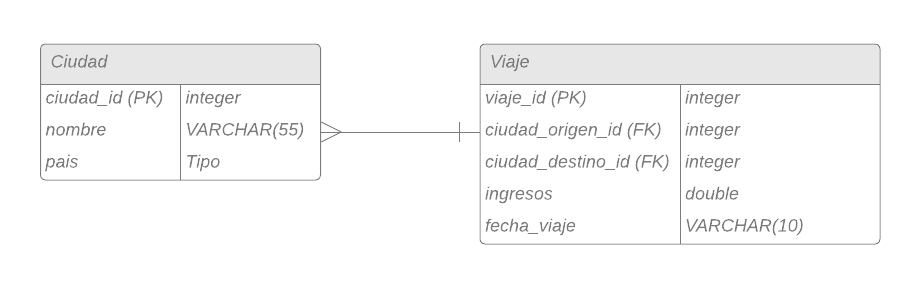
\includegraphics[width=0.8\textwidth]{images/uber_bd.png}
\caption{Tabla de dimensión (Ciudad) y tabla de hechos (Viaje) relacionadas por las columnas \textit{ciudad\_id} y las columnas \textit{ciudad\_origen\_id} y \textit{ciudad\_destino\_id}}. \label{fig:modeloDimensional}
\end{figure}

Una de las posibles consultas que se podrían realizar utilizando ambas tablas es obtener los ingresos totales generados en cada ciudad en un período de tiempo específico, se muestra el código de SQL que se usaría para dicha consulta:

\begin{minted}[
frame=lines,
framesep=2mm,
bgcolor=LightGray,
fontsize=\scriptsize,
linenos
]{sql}
    SELECT
        d.nombre AS Ciudad,
        SUM(v.ingresos) AS IngresosTotales
    FROM
        Viajes v
    JOIN
        Ciudad d 
    ON 
        v.ciudad_destino_id = d.ciudad_id
    WHERE
        v.fecha_viaje BETWEEN '2024-01-01' AND '2024-02-29'
    GROUP BY
        1;
\end{minted}
%\newpage


A simple vista, el contar con dos tablas llevaría a creer que estamos haciendo un uso más costoso de espacio, lo que es correcto. Pero, en caso de que haya que realizar algún tipo de mantenimiento y/o adaptación, este será fácil de gestionar.
Además, de este modo se clarifica la estructura de la base de datos al asignar un propósito claro a cada tabla: las dimensiones proporcionan contexto descriptivo y la tabla de hechos almacena medidas numéricas.

\section{Marcos de trabajo de desarrollo web}\label{sec:framework}

Hoy en día, para el desarrollo y mantenimiento de aplicaciones web se hace uso de los \texttt{Frameworks de desarrollo web}.

Los \texttt{Frameworks de desarrollo web} son un tipo de software diseñado para facilitar el desarrollo de aplicaciones web al proporcionar medios que permiten a los desarrolladores enfocarse en las partes importantes del desarrollo. 

Se encargan de facilitar tareas tediosas como el manejo de sesiones, la localización, la validación de entradas del usuario, formularios, herramientas para la visualización de datos, entre otras aplicaciones con una cantidad mínima de configuración. Esto hace que su uso sea práctico y reusable en el entorno de desarrollo web, ya que los desarrolladores no tienen que crear desde el inicio algunos de los componentes necesarios para un nuevo proyecto \cite{garcia2018analisis}.

Por lo tanto, se puede decir que los propósitos principales para utilizar \textit{Frameworks} son:

\begin{itemize}
    \item Acelerar el proceso desarrollo.
    \item Reusar código existente.
    \item Promover buenas prácticas de desarrollo con el uso de patrones diseño.    
\end{itemize}

Actualmente existen diferentes \texttt{Frameworks de desarrollo web} disponibles en diferentes lenguajes de programación, sin embargo hoy en día los lenguajes más usado para el desarrollo de aplicaciones web son \textbf{JavaScript, Python} y \textbf{Java} \cite{joana_martini}. 

JavaScript es ampliamente utilizado para el desarrollo del  \textit{Frontend}, permitiendo la creación de interfaces interactivas y dinámicas en el navegador web. 
Por otro lado, Python suele ser empleado tanto en el lado del \textit{Backend}, como en el desarrollo de aplicaciones web completas a través de \textit{frameworks} como Django y Flask.  Java también se mantiene como una opción popular, especialmente en grandes empresas.

\subsection{Backend}

El \texttt{Backend} se refiere a la parte de una aplicación web que no es visible para el usuario final, pero que es esencial para su funcionamiento. 

Este se encarga de la configuración de todos los aspectos lógicos de la aplicación; engloba las funciones lógicas, de almacenamiento de datos y de seguridad necesarias para que la aplicación funcione de forma correcta y segura, de modo que todas las acciones solicitadas en la página web se ejecuten correctamente.


Entre sus componentes que conforman el \texttt{Backend} de una aplicación web podemos encontrar los siguientes:

\begin{itemize}
    \item \textbf{Servidores}:
     Se refiere a una máquina física o virtual que gestiona los recursos necesarios para ejecutar una aplicación web. Al recibir las peticiones de los usuarios, los servidores ejecutan la lógica necesaria y devuelven las respuestas a través de un protocolo de comunicación.

     \item \textbf{Lógica de la aplicación}:
     Es la secuencia de operaciones que los desarrolladores programan en el \texttt{Backend} para realizar tareas.

     \item \textbf{Frameworks}:
     Son bibliotecas para el \texttt{Backend} que los programadores utilizan para facilitar la escritura y actualización del código del servidor. Para el \texttt{Backend} existen bibliotecas de procesamiento de datos y herramientas que proporcionan acceso a segmentos de código funcionales.

    \item \textbf{Bases de datos}:
    Contienen la información a la que acceden los servidores para completar las funciones directas de la aplicación y también tienen opciones para clasificar la información a la que pueden acceder diferentes usuarios.
\end{itemize}

Tener un \texttt{Backend} en una aplicación  web proporciona una base sólida para la gestión de datos, la seguridad, la escalabilidad y la eficiencia. También delimita claramente entre la lógica empresarial y la interfaz de usuario, agilizando tanto la gestión como el desarrollo a largo plazo de la aplicación \cite{baker2022secure}.

\subsection{Django}
\texttt{Django} es un \textit{framework} web de Python de alto nivel que fomenta el desarrollo rápido y el diseño limpio y pragmático, este \textit{framework} se basa en el patrón de diseño \textit{Modelo, Vista, Controlador (MVC)}.

\begin{enumerate}
  \item \textbf{Modelo}:  Incluye los datos y el estado de la aplicación web. Se comunica con la base de datos.
  \item \textbf{Vista}: Representa la interfaz visual mostrando la vista seleccionada por el controlador como un HTML. También solicita actualizaciones y prepara datos del modelo.
  \item \textbf{Controlador}: El último componente se comunica con el usuario, gestionando sus peticiones. En función de ellas, envía una petición al modelo y selecciona la vista que debe mostrarse al usuario. Maneja las funcionalidades y la lógica de la web.
\end{enumerate}

Una ejemplificación de como funciona este tipo de arquitectura se puede observar en la Figura \ref{fig:patronDis} dónde el usuario hace una petición la cual es dirigida al \textit{Controlador}, el cual a su vez manda una solicitud al \textit{Modelo} que se comunica con la base de datos para mandar de regreso una solicitud con los datos al \textit{Controlador}, el cual por último manda una solicitud a la \textit{Vista} la cual regresa una respuesta al usuario.\\

%\textcolor{red}{Explicar Figura \ref{fig:patronDis}patron de diseño}

%\newpage
%\begin{center}
    \begin{figure}[H]
        \centering
        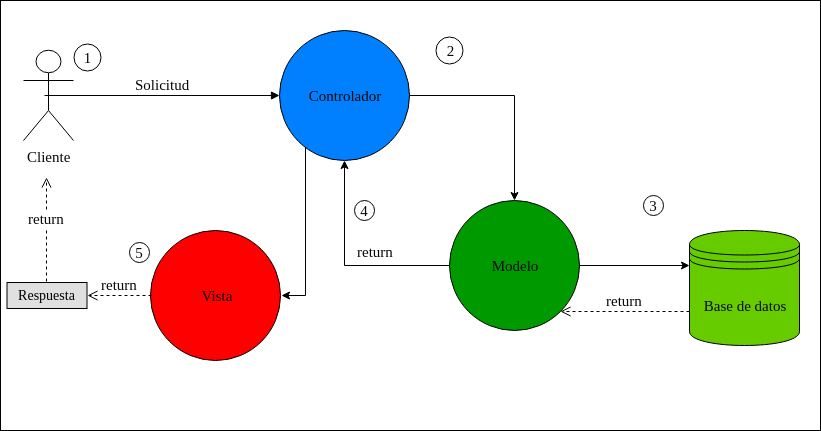
\includegraphics[width=0.6\textwidth]{images/MVC.png}
        \caption{Diagrama del funcionamiento del patrón de diseño \textit{MCV}} \label{fig:patronDis}
    \end{figure}
%\end{center}

Hay amplias razones por las que hoy en día este \textit{framework} web es elegido para desarrollar aplicaciones web, en concreto la parte correspondiente al \textit{Backend}. Al explorar lo que ofrece, se puede observar que es extremadamente rápido y escalable, seguro y versátil, lo que lo convierte en una herramienta para el desarrollo rápido de aplicaciones web haciendo uso de código limpio y fácil de mantener \cite{baker2022secure} \cite{gagliardi2021decoupled}.

Entre sus características, podemos encontrar las siguientes \cite{django}:
\begin{itemize}
    \item \textbf{Mapeador objeto-relacional (ORM, Object-Relational Mapper)}\\
    El ORM de Django permite a los desarrolladores interactuar con la base de datos usando código de Python, en lugar de escribir SQL en bruto. Esto hace que sea fácil trabajar con diferentes bases de datos y cambiar entre ellas si es necesario.

    \item \textbf{Interfaz de administración automática} \\
    Django proporciona una interfaz de administración incorporada que facilita la gestión de datos.
    
    \item \textbf{Sistema de plantillas}\\
    Django proporciona un dinámico sistema de plantillas que permite separar la representación de los datos de la lógica de la aplicación.

    \item \textbf{Enrutamiento URL}\\
    Django proporciona un eficaz sistema de enrutamiento de URLs que facilita la asignación de URLs a vistas.
    
\end{itemize}

Hablando en términos de escalabilidad, Django está probado y es escalable. Es utilizado por algunos sitios de tráfico pesado como Eventbrite, Disqus, Instagram, Prezi, Pinterest y Washington Post. Además, Django se puede acoplar con diferentes tecnologías como \textit{ReactJS} para el libre desarrollo de los proyectos que hacen uso de este \textit{framework} \cite{gagliardi2021decoupled}.

\subsection{Frotend}

En épocas pasadas, las páginas web se asemejaban a la estática disposición de las páginas de un libro, presentando información de manera fija y limitada. Este enfoque estático, sin embargo, distaba de satisfacer las expectativas de la experiencia moderna en la web.

Esencialmente, hoy en día una página web se compone de lenguaje de marcado de hipertexto (\textbf{HTML}), hojas de estilo en cascada (\textbf{CSS}) y \textbf{JavaScript}. El HTML define la estructura de una página web, el CSS estiliza la página, y JavaScript permite las interacciones del usuario. Los tres combinados se consideran desarrollo web \texttt{Frontend}.

Pero el desarrollo \texttt{Frontend} no sólo abarca el diseño y lógica de la aplicación. La responsividad y el rendimiento son los dos objetivos principales del \texttt{Frontend}. Un desarrollador debe asegurarse de que el sitio sea responsivo, es decir, que aparezca correctamente en dispositivos de todos los tamaños: ninguna parte del sitio web debe comportarse de forma anómala independientemente del tamaño de la pantalla \cite{wieruch2018road}.

Como se mencionó, \textbf{JavaScript} es el lenguaje encargado de las interacciones que los usuarios realicen; es un lenguaje de programación que los desarrolladores utilizan para hacer páginas web interactivas. Desde actualizar fuentes de redes sociales a mostrar animaciones y mapas interactivos, las funciones de \textbf{JavaScript} pueden mejorar la experiencia del usuario de una página web.\\
Adicionalmente, existen diversos \textit{frameworks} y bibliotecas para \textbf{JavaScript} que facilitan el desarrollo de aplicaciones web, algunos ejemplos son \textit{ReactJS}, \textit{AngularJS} y \textit{jQuery}.

\subsection{Visualización de datos}

El propósito principal de este trabajo es ayudar a \textbf{SEDESA} a analizar los datos provistos y mostrarlos en diferentes gráficas, pero el uso de gráficas no se limitaría únicamente a este módulo, también se usaría en diferentes módulos que quedan fuera del alcance de este trabajo. Para esto se debía hacer uso de gráficas de barras, barras empiladas, pastel, series de tiempo, mapas coropléticos y tablas \cite{grant2018data} \cite{hinderman2016building} \cite{kirk2016data}.

Se exploraron diferentes bibliotecas de \textbf{JavaScript} que se podrían usar para la generación de gráficas. Se consideraron bibliotecas \textit{Open Source} y en las cuales se debían pagar una licencia por su uso.
La elección de la biblioteca para la visualización de datos no sólo se basó en sus capacidades técnicas, sino también en consideraciones de licencia. Se evaluaron las bibliotecas en términos de su adecuación para el proyecto, su compatibilidad con el flujo de trabajo y los requisitos de licencia asociados. Se buscó equilibrar la funcionalidad necesaria con la viabilidad económica y la alineación con los principios de código abierto cuando fuera posible.
En la Tabla \ref{tab:biblioVis} se presenta una comparativa de las bibliotecas de visualización de datos consideradas.

\begin{table}[!htb]
\small
    \centering
    \resizebox{\textwidth}{!}{%
        \begin{tabular}{ |p{2.2cm}|p{2.4cm}|p{4cm}|p{4cm}|  }
            \hline
            \textbf{Biblioteca} & \textbf{Software \textit{Open source}} & \textbf{Ventajas} & \textbf{Desventajas} \\
            \hline
            ChartJS & Sí & \begin{itemize}[left=0pt]
              \item Gráficas dinámicas y responsivas con un render de los valores previamente.
              \item Se maneja con canvas que da mejor rendimiento que SVG.
              \item Las gráficas se pueden descargar como imágenes.
              \item Se pueden configurar las gráficas.
              \item La curva de aprendizaje es sencilla.
            \end{itemize} & \begin{itemize}[left=0pt]
                \item Suele usarse para proyecto de menor escala.
            \end{itemize}. \\

            \hline
            D3 JS & Sí & \begin{itemize}[left=0pt]
                          \item Permite crear gráficos de vector.
                          \item Manejo de datos CSV, JSON y otros formatos.
                          \item Interacción con gráficos (zoom, desplazarse, arrastrar).
                          \item Manejo de datos geográficos.
                        \end{itemize} & \begin{itemize}[left=0pt]
                                            \item Se necesitan bibliotecas adicionales para exportar gráficos.
                                            \item La curva de aprendizaje es compleja.
                                          \end{itemize} \\
            \hline
            
            HighCharts & No & \begin{itemize}[left=0pt]
                                  \item Gran cantidad de gráficos dinámicos.
                                  \item Soporte técnico al obtener la licencia.
                                  \item Curva de aprendizaje intermedia por la gran documentación.
                                \end{itemize} & \begin{itemize}[left=0pt]
                                                    \item Para obtener todas las ventajas hay que pagar licencia.
                                                    \item Se cobra licencia por cada desarrollador que modificará la página.
                                                  \end{itemize} \\
            \hline
            
            AmCharts & No & \begin{itemize}[left=0pt]
                               \item Gráficas responsivas, interactivas y dinámicas.
                               \item La curva de aprendizaje es media.
                               \item Panel y modelos personalizables.
                             \end{itemize} & \begin{itemize}[left=0pt]
                                               \item Es libre para desarrollo, sin embargo se debe pagar licencia para integrarlo al proyecto.
                                             \end{itemize} \\
            \hline
        \end{tabular}%
    }
    \caption{Bibliotecas de visualización de datos} \label{tab:biblioVis}
\end{table}

Una vez hecho el análisis comparativo entre cada bibliotecas se llegaron a las siguientes conclusiones de acuerdo a cada biblioteca:

\begin{itemize}
    \item ChartJS es muy intuitivo de utilizar, responsivo y fácil de implementar, sin embargo, cuenta con gráficas básicas como líneas, barras y pie, pero dentro de los requerimientos surge la necesidad de utilizar mapas y aquí es donde carece esta biblioteca \cite{chartjs_docs}.

    \item D3JS tiene una amplia comunidad que le da soporte constantemente a los gráficos desarrollados en esta biblioteca, sin embargo, la curva de aprendizaje a utilizar es más amplia para el tiempo reducido que se cuenta para el proyecto. Su implementación requiere un cantidad líneas de código grande para una gráfica en apariencia sencilla, y su personalización es demasiado compleja \cite{d3js_what_is_d3}.

    \item La biblioteca de HighCharts, además de estar enfocado en móviles y finanzas, también cuenta con características de navegación en altos volúmenes de información, anotaciones de usuarios y algunos indicadores técnicos, que si bien, harían que dichas gráficas tengo una mejor calidad en la presentación final, generan un aumento considerable en el costo final de la licencia, por lo que, al menos que se tenga la solvencia liberada para el proyecto, no sería de uso fundamental para el desarrollo de los tableros \cite{highcharts}.

    \item AmCharts ofrece el mismo tipo de gráficas que HighCharts, siendo la gran diferencia el costo de la licencia y el hecho de qué al adquirir la licencia no existe un límite de desarrolladores que interactúen en la misma aplicación interna \cite{amcharts_about}.
\end{itemize}


\subsection{AmCharts}

Después de juntas con representantes de \textbf{SEDESA} dónde expusieron las necesidades del proyecto en cuánto al tipo de gráficas que se necesitarían y comparándolo con las bibliotecas anteriormente mencionadas, se decidió optar por el uso de \texttt{AmCharts} en su versión 5.

Entre sus características más notorias se pueden mencionar las siguientes:

\begin{itemize}
    \item \textbf{Procesamiento de datos rápido}\\
    El procesamiento de datos dentro de \texttt{AmCharts 5} está diseñado para ser lo más eficiente posible. Las actualizaciones incrementales, la ausencia de agregaciones repetitivas y el uso de objetos de datos ligeros hacen que el procesamiento de datos sea rápido y eficiente en términos de memoria.

    \item \textbf{Plantilla de elementos}\\
    La mayoría de los elementos se crean utilizando plantillas: una colección de ajustes, eventos y adaptadores predeterminados. Al cambiar de plantilla, los cambios se propagan automáticamente a los elementos reales, lo que facilita las actualizaciones por lotes.

    \item \textbf{Estado de los elementos}\\
    La biblioteca permite cambiar fácilmente el aspecto de un elemento en diferentes circunstancias, por ejemplo, en alguna interacción, hover, clic, o en relación con los datos (por ejemplo, el aspecto de una columna si un valor está abajo).
    El motor aplicará automáticamente las propiedades requeridas según sea necesario, animando entre los valores antiguos y nuevos suavemente.
\end{itemize}

A partir del análisis realizado se puede decir que, \texttt{AmCharts 5 }es una robusta biblioteca de visualización de datos que ofrece un variado conjunto de opciones de visualización. 
Admite gráficas tradicionales como líneas, áreas, columnas, dispersión, entre otras, con la flexibilidad de combinar estos tipos. También incluye gráficas porcentuales, circulares, de dona, mapas geográficos y visualizaciones especializadas como diagramas de Sankey, mapas de árbol, nubes de palabras y diagramas de Venn. Además, la biblioteca incluye funciones avanzadas como diagramas de Gantt, diagramas de cascada y visualizaciones de libro de pedidos/profundidad. Con opciones adicionales como diagramas de acordes, sunbursts e histogramas radiales, AmCharts 5 es una herramienta versátil para crear una amplia gama de visualizaciones de datos atractivas e informativas \cite{amcharts_about}.


%-------------------------------------------------------------------
\section{Resumen}

%En este capítulo se expusieron la terminología y conceptos relacionados con ....



En este capítulo, se ha explorado y contextualizado la terminología y los conceptos fundamentales relacionados con la implementación del tablero de datos solicitado. Se abordaron conceptos esenciales que abarcan desde la elección de la base de datos y su modelo relacional hasta la selección del sistema de gestión de bases de datos, haciendo hincapié en la importancia del lenguaje \texttt{SQL} en este contexto.

Además, se proporcionó una visión detallada de la elección de \texttt{PostgreSQL} como sistema de gestión de bases de datos, destacando su versatilidad y adaptabilidad. 
Se discutió la relevancia de los \textit{frameworks} de desarrollo web, centrándose en \texttt{Django} como una herramienta eficaz para el desarrollo del \textit{backend} de aplicaciones web.

La subsección dedicada a la visualización de datos examinó diversas bibliotecas de JavaScript, detallando sus ventajas y desventajas. Tras una exhaustiva comparación, se optó por el uso de \texttt{AmCharts 5} debido a su capacidad para generar gráficas dinámicas, responsivas e interactivas, además de su flexibilidad y versatilidad en términos de visualización de datos, costo y libertad para el uso dentro del equipo de trabajo.

En conclusión, este capitulo busca informar al lector de todas las tecnologías usadas para la implementación del tablero, se buscó dar a entender las diferencias, ventajas y desventajas de usar tecnologías \textit{Open source} como lo son \texttt{Django} y \texttt{PostgreSQL} en comparación con tecnologías dónde se debe hacer la compra de la licencia para usarla como lo es \texttt{AmCharts}.
%Estado del arte

\chapter{Estado del arte}\label{cap:edoarte}

%Que se está utilizando en la literatura o en el mercado para implementar tableros de datos
%Hablar de software Open Source y de paga mencionando ventajas y desventajas de cada uno. También explicar porque cada software no es viable para la solución.

El presente capítulo tiene como objetivo realizar una revisión crítica y sistemática de la literatura y el mercado actual en torno a la implementación de tableros de datos. Se analizará el uso de software \textit{Open Source} y de pago, considerando sus ventajas y desventajas, con el fin de determinar la mejor opción para la implementación de un tablero de datos en el contexto del presente trabajo.\\

Se presentará una revisión de las principales herramientas \textit{Open Source} disponibles para la creación de tableros de datos, como Tableau Public, Google Data Studio y Grafana. Se describirán sus características, ventajas y desventajas. De manera similar, se analizarán las principales herramientas de pago disponibles para la creación de tableros de datos, como Microsoft Power BI, Tableau y Domo.



\section{Software para tableros de datos}\label{sec:seccion3.1}
Un software para la implementación de tableros de datos, es una plataforma centralizada que permite a las empresas e instituciones visualizar y analizar información compleja de forma simplificada e intuitiva. Ayudan a presentar los datos en un formato visualmente atractivo e interactivo, lo que permite a los usuarios supervisar los indicadores clave de rendimiento \textit{(KPI)} y obtener información procesable para tomar decisiones informadas \cite{wexler2017big}.

En esencia, este tipo de software actúa como puente entre los datos brutos y la información significativa. Transforma conjuntos de datos complejos en representaciones visuales comprensibles. Esto facilita a los usuarios la comprensión e interpretación de la información. Los tableros suelen consistir en diagramas, gráficos, tablas y otros elementos visuales que condensan grandes volúmenes de datos en visualizaciones concisas y significativas \cite{kirk2016data} \cite{kerzner2015dashboard}. \\

Las principales características que se buscan en un software para el desarrollo de tableros son las siguientes \cite{wexler2017big}:

\begin{enumerate}
    \item \textbf{Plantillas de tableros predeterminadas y opciones de estilos}\\
    Esta característica permite a los usuarios elegir entre plantillas prediseñadas y personalizar el estilo del tablero para adaptarlo a sus necesidades.
    
    \item \textbf{Seguridad de los datos}\\
    Este es un aspecto importante a tener en cuenta antes de elegir la herramienta adecuada. Garantizar que los datos confidenciales de la institución están protegidos en todo momento es de gran importancia, no sólo por razones de seguridad, sino también porque las normativas de seguridad son cada vez más estrictas.
    
    \item \textbf{Procesamiento de datos en tiempo real}\\
    Un tablero tiene como uno de sus propósito proporcionar las tendencias generales al tiempo que permite a los usuarios la capacidad de desglosar y acceder a múltiples capas de datos.
    
    \item \textbf{Personalización e integración}\\
    Un tablero que puede ser personalizable permite a los usuarios elegir qué puntos de datos y visualizaciones pueden ver, mientras que la integración con otras herramientas permite mejorar los análisis e informes.

    
    \item \textbf{Gráficos}\\
    Un buen software para desarrollo de datos debe de proporcionar gráficas personalizables que ayudan a transmitir las métricas esenciales de forma rápida y atractiva.

    \item \textbf{Opciones para compartir}\\
    Un buen software suele proveer diversas opciones para compartir tableros entre diferentes personas. Esto se puede hacer mediante el inicio de sesión desde otro dispositivo, el envío de tableros e informes por correo electrónico, o el uso de un visor externo.

    \item \textbf{Capacidad de exportación e impresión}\\
    Esta característica permite poder exportar los tableros en archivos con formato PDF o PNG sin que el tablero pierda su estructura y diseño al momento de la conversión.
    
    
\end{enumerate}





\section{Software Open Source}
La implementación de tableros de datos utilizando tecnología de código abierto tiene muchas ventajas que los convierten en una opción sustentable para muchas organizaciones. A continuación se analizarán algunas de los principales software \textit{open source} que se utilizan para la creación tableros de datos creados con tecnología de código abierto, junto con ejemplos de algunos de los principales casos de uso para los que se ha utilizado dicha tecnología.

\subsection{Tablueau Public}
Tableau Public es una plataforma gratuita para explorar, crear y compartir públicamente tableros para la visualización de datos en línea. Cualquier persona puede crear tableros utilizando la aplicación web.\\
Se pueden procesar datos en diversos formatos, como Excel, CSV y Google Sheets, para crear visualizaciones atractivas e interactivas con una interfaz fácil de usar la cual no requiere de la producción de código \cite{tableau_public_about}.\\

La razón principal por la cual esta opción no es viable para la implementación de este proyecto, se debe a que los datos pueden ser observados por cualquier persona, lo cual no de debería ser posible ya que se manipulan datos privados y delicados que no son de uso público.

\subsection{Grafana}
Grafana es una aplicación web de análisis y visualización interactiva multiplataforma. Proporciona tablas, gráficas y alertas para la web cuando se conecta a fuentes de datos compatibles. Es principalmente una herramienta de visualización que proporciona gráficos interactivos para administradores y tableros de datos alimentados por flujos de entrada de datos.\\
Grafana cuenta con un modelo de fuente de datos conectable que puede conectarse con una amplia gama de fuentes de datos, incluidos datos de series temporales, pero también bases de datos relacionales como lo MySQL y PostgreSQL \cite{mccollam2022getting}.\\

La razón por la cual se descartó su uso para este proyecto se debe la curva de aprendizaje es grande. La configuración de los plugins puede requerir un esfuerzo considerable. Las opciones de configuración a través de la interfaz gráfica de usuario son limitadas y a menudo es necesario el mantenimiento y la edición manual de los archivos de configuración.


\subsection{Google Data Studio}
Google Data Studio es una herramienta de \textit{Business Intelligence (BI)}, que procesa datos brutos en información estratégica para las empresas e instituciones. A través de la visualización de datos, Google Data Studio reúne métricas e indicadores que apoyan la toma de decisiones y estrategias. Está diseñada para ayudar a los profesionales del marketing, a los propietarios de empresas y a los analistas de datos a visualizar los datos para obtener información y tomar decisiones fundamentadas. Google Data Studio es compatible con más de 150 fuentes de datos, como Google Analytics, Google Ads, Google Search Console, BigQuery, YouTube Analytics y muchas otras \cite{kemp2021google}.\\
Además, esta plataforma permite hacer operaciones sobre los datos al momento de exportarlos. Por ejemplo, si tenemos una columna dónde los datos son fechas en formato \texttt{Unix Timestamp} o en días (DD/MM/YYYY) y el objetivo es mostrar una serie de tiempo, pero agrupada en meses o años, Google Data Studio provee opciones para hacer este tipo de operaciones y más, como la posibilidad de modificar interactivamente los tableros mediante filtros.\\

La razón por la cual no se decidió trabar con este producto de Google se debe a qué es relativamente nuevo y no cuenta con todo el tipo de gráficas que se necesitan para el proyecto y la personalización de estas es limitado.
%-------------------------------------------------------------------


\section{Software de paga}
Habiendo hablado de opciones \textit{Open source} las cuales proveen herramientas provechosas para la implementación y creación de tableros de datos, estas tecnologías son una gran opción si el proyecto en el que se está trabajando no es de una escala considerablemente grande, los datos que se manipulan no son privados o los encargados de la implementación no cuentan con una amplia experiencia en cuestión de programación o con el uso de \texttt{SQL}.\\
Ya que como se pudo observar, todas las opciones mencionadas tienen algún tipo de restricción en cuanto a lo que concierne al proyecto en el que se trabajó. Los datos desplegados en el tablero de datos no son de uso público y las herramientas \textit{Open source} no permiten una personalización extensa.\\

En esta sección se explorarán herramientas por las cuales hay que realizar algún tipo de pago para usarlas, las cuales pueden llegar a ofrecer servicios más extensos y personalizables que los anteriormente vistos.


\subsection{Microsoft Power BI}
Power BI es un conjunto de servicios de software, aplicaciones y conectores que trabajan juntos para convertir diferentes fuentes de datos no relacionadas en perspectivas coherentes, visualmente inmersivas e interactivas. Los datos pueden estar contenidos en una hoja de cálculo de Excel o una colección de almacenes de datos híbridos basados en la nube y locales. Power BI  permite conectarse fácilmente a sus fuentes de datos, visualizar y descubrir lo que es importante, y compartirlo con quien se desee \cite{microsoft_power_bi_overview} \cite{clark2017beginning}.\\

En la Figura \ref{fig:powerBI_ej} se puede observar un tablero de datos con diferentes métricas y datos sobre ventas y marketing, implementado en \texttt{Power BI}.

%\begin{center}
    \begin{figure}[H]
        \centering
        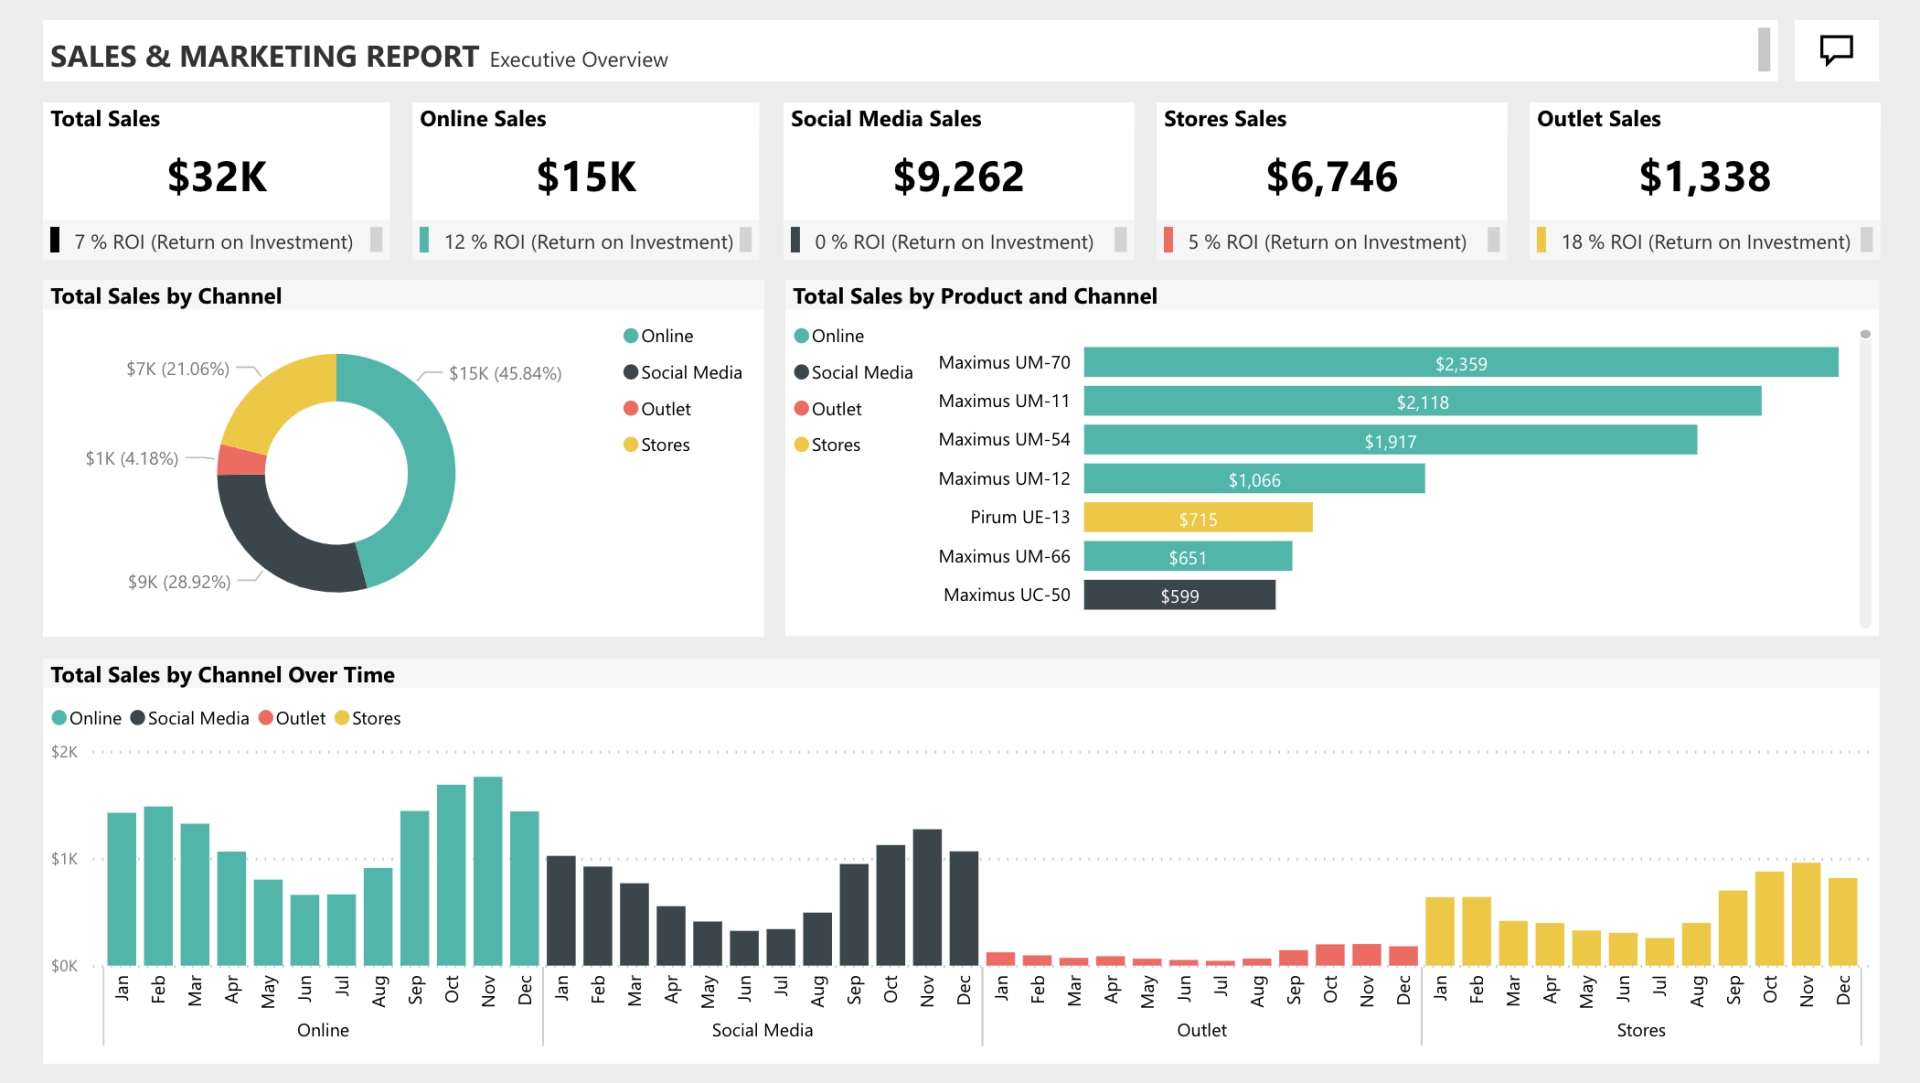
\includegraphics[width=0.8\textwidth]{images/power_bi_ejemplo.png}
        \caption{Ejemplo de un tablero de datos implementando en \texttt{Power BI}.}\label{fig:powerBI_ej}
    \end{figure}
%\end{center}

Una de las características más notorias de este servicio es que puede usar tanto en su página web, en su aplicación local para computadoras y su aplicación para dispositivos móviles Android y iOS. Además de que se puede usar en conjunto con los diferentes productos que Microsoft ofrece.\\
Un diferenciador que resalta bastante en comparación a otros software es que los usuarios de Power BI  pueden acceder al reconocimiento de imágenes y al análisis de texto, crear modelos de aprendizaje automático e integrarse con Azure Machine Learning para ampliar el valor de sus análisis mediante potentes capacidades de \textit{Machine Learning} y/o \textit{Inteligencia Artificial}.\\

En cuánto a la capacidad de personalización de tableros de datos, Power BI provee una gran libertad para personalizar los tableros al ofrecer una gran cantidad de gráficas y combinación de temas para el canvas.\\

Uno de los servicios de Power BI más interesantes y útiles al momento de analizar los datos que se manipulan, es el servicio de \textbf{Natural Language Q \& A Question Box (Caja de preguntas mediante procesamiento de lenguaje natural)} \cite{ivision_power_bi_usage}.\\
Esta función de Power BI permite escribir una pregunta en el cuadro \textit{Formule una pregunta sobre los datos} para obtener rápidamente respuestas a partir de sus datos. Power BI utiliza funciones cognitivas como la reformulación, el autorrelleno y las sugerencias para obtener resultados de búsqueda de inmediato, en la Figura \ref{fig:power_bi_nlp} se puede ver un ejemplo de como se muestra esta función en Power BI.\\
Power BI busca las mejores respuestas basándose en un conjunto de datos e informes preconfigurados. Incluso elige la mejor visualización para mostrar las respuestas de la forma más útil.
Con el uso de esta función, los usuarios ahorran tiempo. Power BI también  permite guardar las preguntas más frecuentes para que otros usuarios puedan consultarlas fácilmente.\\

%\newpage

%\begin{center}
    \begin{figure}[H]
        \centering
        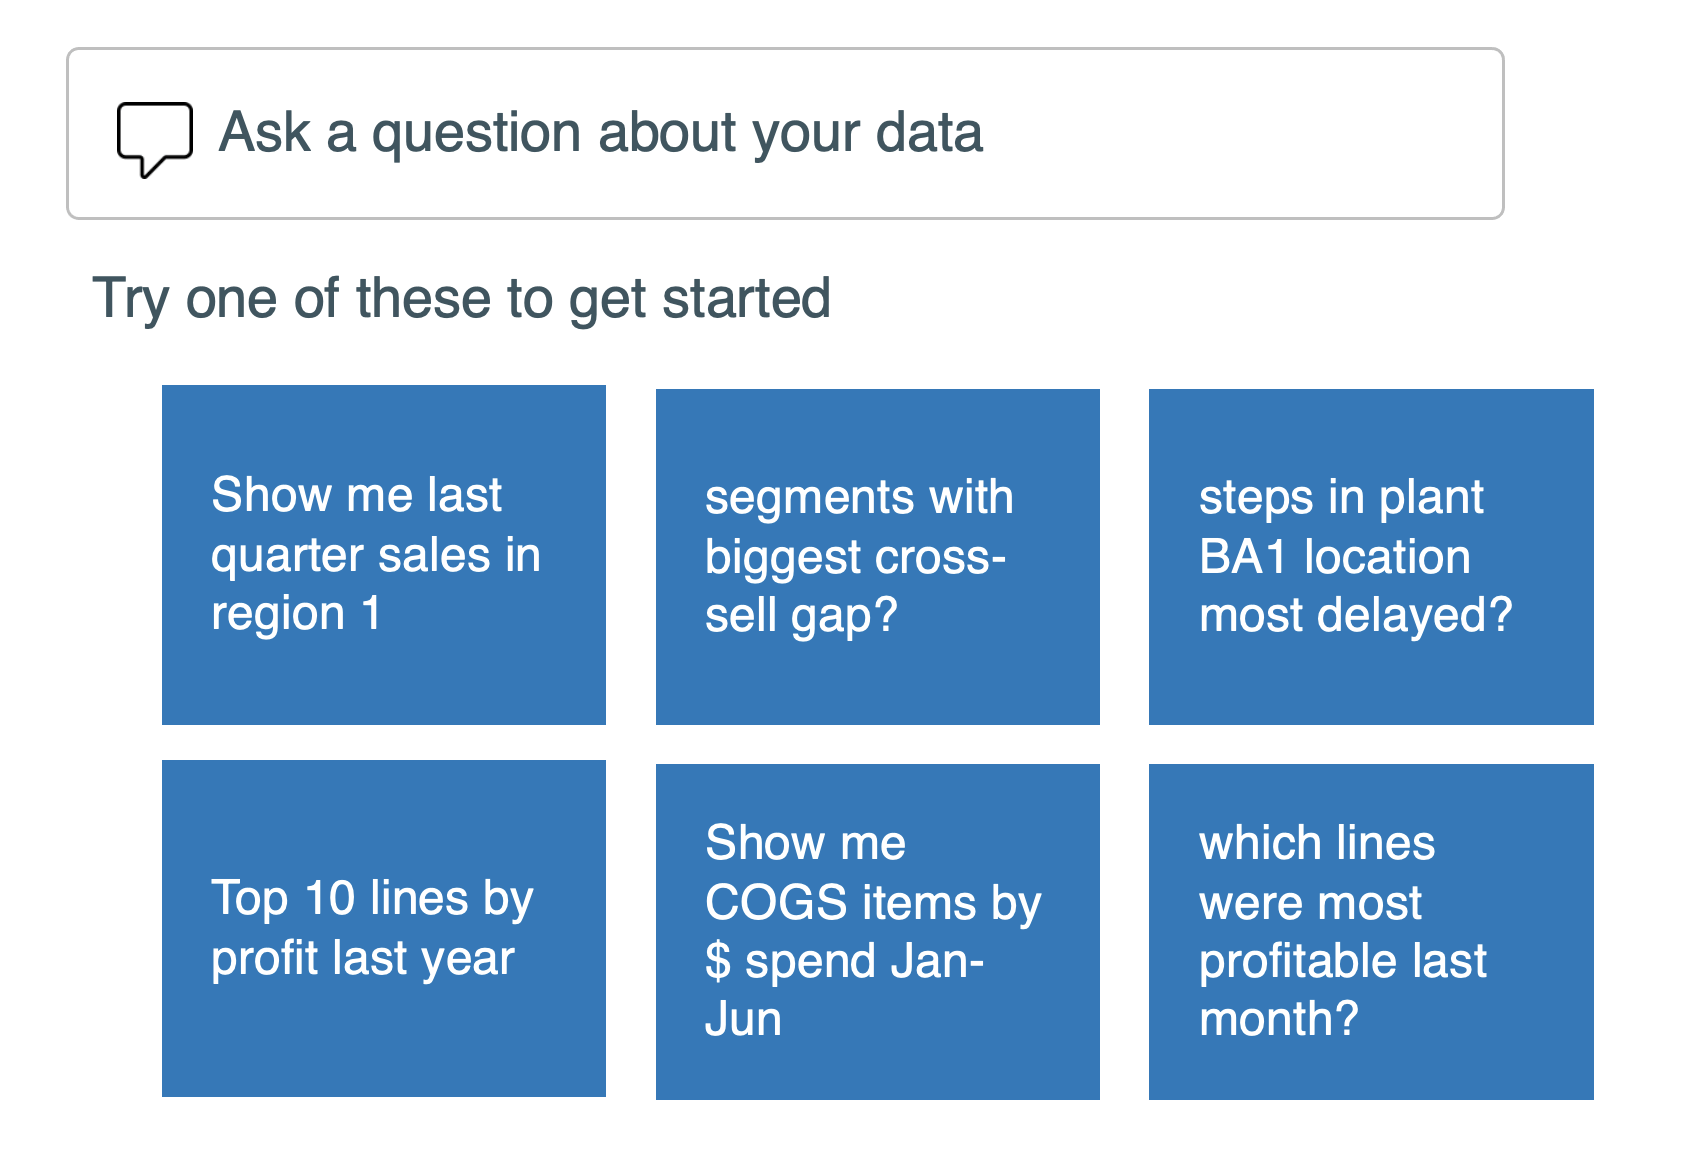
\includegraphics[width=0.6\textwidth]{images/power_bi_Q&A.png}
        \caption{Ejemplo de uso de la función Question Box de \texttt{Power BI}.} \label{fig:power_bi_nlp}
    \end{figure}
%\end{center}

Las razones por las cuales no se hizo uso de Power BI es debido a que en el proyecto no se tienen integrados productos de Microsoft mas que GitHub, lo cual no le quita valor a todo lo que Power BI ofrece, pero se podría hacer un uso más provechoso si en el proyecto se trabajara con un \textit{stack} más enfocado en productos de Microsoft como Azure. Además el costo por una licencia individual para un desarrollador va desde 211 hasta 422 pesos mexicanos, lo cual no es algo que verdaderamente convenga pagar para este tipo de proyecto y las licencias para organizaciones, su precio varias dependiendo de las necesidades. Por último, \textbf{SEDESA} solicitó que todos los módulos del proyecto se encuentren en un mismo sitio, es decir, que se puedan acceder de manera sencilla, por lo que tener únicamente el tablero en una plataforma diferente no es lo más apropiado dado los requerimientos del proyecto.

\subsection{Tableau}
Tableau es una herramienta líder de Business Intelligence (BI) y visualización de datos, diseñada para hacer que el análisis de datos sea accesible e intuitivo para usuarios de distintos niveles. Permite a individuos y organizaciones transformar datos en crudo en tableros de datos interactivos y compartibles, proporcionando información que impulsa la toma de decisiones informadas.\\
A diferencia de las herramientas para creación de tableros de datos, que requieren amplios conocimientos técnicos, Tableau busca dar prioridad a la facilidad de uso, lo que permite a los usuarios técnicos y no técnicos crear visualizaciones y análisis complejos con facilidad, en la Figura \ref{fig:tableua_workload} se muestra como funciona el flujo de trabajo de Tableau. Es compatible con una amplia gama de fuentes de datos, desde hojas de cálculo y bases de datos hasta servicios en la nube, lo que garantiza flexibilidad y conectividad \cite{tableau_help_use_cases} \cite{costello2020prepare}.

\begin{figure}[H]
    \centering
    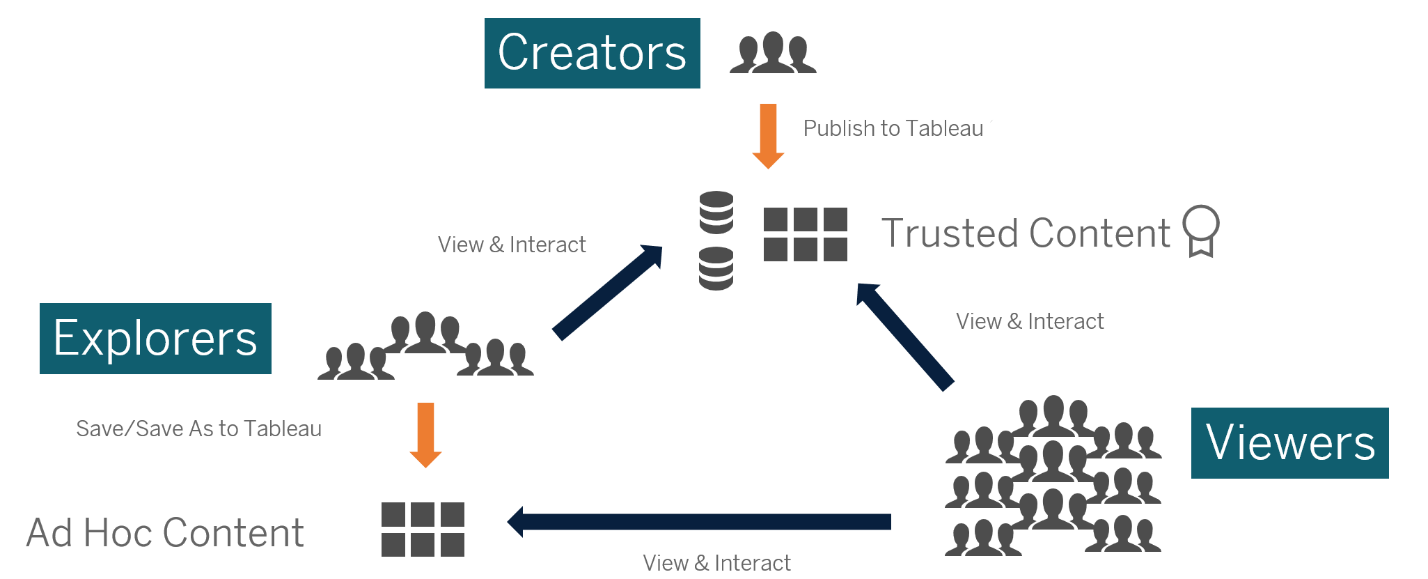
\includegraphics[width=0.7\textwidth]{images/bp_use_cases_1.png}
    \caption{Diagrama del funcionamiento de \texttt{Tableau}.} \label{fig:tableua_workload}
\end{figure}

Entre las características de Tableau, se pueden encontrar las siguientes:
\begin{itemize}
    \item Tableau cuenta con más de 100 conexiones de datos integradas que van desde archivos de texto como Excel a bases de datos como PostgreSQL o herramientas en línea como Google Analytics o Salesforce.com.

    \item Tableau provee una interfaz amigable con el usuario basada únicamente en las acciones de arrastrar y soltar, la interfaz de usuario permite crear fácilmente cuadros, gráficos, mapas y otras visualizaciones sin necesidad de amplios conocimientos previos en programación.

    \item Los usuarios pueden crear visualizaciones dinámicas y atractivas que permiten a los espectadores explorar interactivamente los datos a través de filtros, capacidades de desglose y parámetros personalizables.

    \item Tableau proporciona funciones estadísticas incorporadas, como regresiones lineales, coeficientes de correlación y desviaciones estándar, lo que permite realizar análisis más avanzados dentro de la propia plataforma si es que así se desea.

    \item De manera similar a Power BI, Tableau también ofrece un función que usa procesamiento de lenguaje natural para hacer preguntas sobre los conjuntos de datos que se manipula.

    \item La función que podría ser considera la más útil y atrayente de Tableau, es el poder combinar datos de diferentes fuentes \cite{tableau_help_multiple_connections}. Por ejemplo, combinar datos que se encuentran contenidos en un hoja de calculo de Excel y diferentes datos que se encuentran en PostgreSQL.

    Existen varias formas de combinar datos, cada una con sus propios puntos fuertes y débiles.

    \begin{itemize}
        \item Las relaciones son el método por defecto y pueden utilizarse en la mayoría de los casos, incluso entre tablas con distintos niveles de detalle.

        \item Las uniones combinan tablas añadiendo más columnas de datos a través de estructuras de filas similares. Esto puede provocar la pérdida o duplicación de datos si las tablas tienen diferentes niveles de detalle.

        \item Las mezclas, a diferencia de las relaciones o las uniones, nunca combinan los datos directamente. En su lugar, las mezclas consultan cada fuente de datos de forma independiente, agregan los resultados al nivel adecuado y, a continuación, los presentan juntos visualmente en la vista.
    \end{itemize}

\end{itemize}

Como se puede observar Tableau es un software bastante poderoso que ofrece una amplia gama de herramientas y facilidades para la implementación de tableros datos y distintas visualizaciones.\\
Es una excelente herramienta que se pudo haber utilizado para el desarrollo de este trabajo, pero como se mencionó en el primer capitulo los recursos asignados para la compra de software de pago es limitado y Tableau cuenta con precios de licencias por desarrollador elevados los cuales van desde los 15 hasta los 75 dolares mensuales. De manera similar a lo mencionado anterior anteriormente con Power BI, todos los módulos solicitados por \textbf{SEDESA}, los cuales no se limitan solamente a la visualización de datos, deben estar localizados dentro una misma aplicación o software.

\subsection{Domo Business Intelligence}
Domo es una plataforma analítica en la nube creada para grandes y pequeñas empresas. Está adecuadamente equipada para cualquier tipo de institución debido a su amplio conjunto de funciones que cubren todos los requisitos que un software de visualización de datos debe cubrir; de seguridad, gobernanza, tableros de datos y generación de reportes, todo ello en un entorno colaborativo. Domo tiene un paquete de gestión empresarial que se integra con múltiples fuentes de datos que ayudan a las instituciones a tomar decisiones cruciales a través de los servicios que Domo tiene para ofrecer \cite{robb2022domo}.\\

Domo posee funciones similares a las ya mencionadas en Tableau y Power BI, pero además de estas, las principales funciones que lo diferencian de sus competidores son las siguientes \cite{graphable_domo_analytics}:

\begin{itemize}
    \item \textbf{Transformación de datos (Ingeniería de datos)}\\
    Domo contiene funciones enfocadas en la Ingeniería de datos para hacer operaciones con los datos manipulados como Magic ETL \footnote{ETL es el acronimo correspondiente al término \textit{Extract, Transform and Load}} (flujos ETL de arrastrar y soltar), SQL dataflows (flujos de datos creados a partir de scripts de SQL) y vistas interactivas de conjuntos de datos están siempre disponibles, todo estos flujos de datos pueden ser creados a partir de varias fuentes de datos desde Google Sheets, MySQL y servicios en la nube como Amazon Web Services. También cuenta con estudio de ciencia de datos, aprendizaje automático automatizado, catálogo de instancias visual/en tiempo real e interactivo, lo cual permiten a los usuarios realizar de tableros y/o visualizaciones de datos de manera más rápida y eficaz.

    
    \item \textbf{Elaboración de Informes y Tableros de Datos}\\
    Domo ofrece una extensa variedad de recursos para la visualización de datos, que incluyen más de 150 tipos de gráficos, más de 7,000 opciones de mapas personalizables, capacidades de análisis mediante la función de arrastrar y soltar, así como la creación de contenido con cálculos personalizados. Estos elementos pueden ser compartidos de manera simple, y la implementación de tableros de datos se realiza de manera sencilla.

    \item \textbf{Creación de aplicaciones interactivas}\\
    Domo provee un servicio para crear aplicaciones interactivas las cuales pueden ser modificadas a partir de la producción de código y/o sin la necesidad de la programación en ReactJS, estas permiten a los usuarios ir más allá del conjunto de visualizaciones y tableros de datos estándar para capturar visualmente incluso los procesos empresariales más específicos y complejos, aprovechando al mismo tiempo todas las capacidades de Domo, incluidas la gobernanza y la seguridad.

    \item  \textbf{Compatibilidad con dispositivos moviles}\\
    Domo también está disponible para dispositivos moviles tanto en iOS como en Android. Tal vez, implementar y desarrollar proyectos en este tipo de dispositivos no es lo más conveniente y eficaz, pero la portabilidad que estos conceden al momento de presentar tableros y/o visualizaciones es poderoso. 
    
    
\end{itemize}

Existen ejemplos en linea dónde se puede observar la capacidad de uso de Domo, desde simples tableros de una sola página no interactivos, hasta aplicaciones interactivas de varias páginas:

\begin{itemize}
    \item En la página \url{https://www.domo.com/dashboard/marketing} ofrece un ejemplo de de como se podría implementar un tablero de datos especializado en marketing que brinda a los usuarios una herramienta para la integración, transformación, análisis y visualización de datos de manera eficiente y efectiva. Este tablero está diseñado específicamente para mostrar como un Domo puede usarse para implementar un tablero de datos que puedan cubrir las necesidades de los profesionales del marketing al proporcionar una visión completa y en tiempo real del rendimiento de sus campañas y estrategias, esto gracias al uso de diversas gráficas que van desde tablas, hasta mapas geográficos, todos ellos personalizados de manera avanzada.
\end{itemize}

Como se puede observar Domo es una gran herramienta que proporciona una diversa cantidad de funciones para la implementación de tableros de datos, siendo más permisiva que Tableau y Power BI en cuestión de personalización.\\
Una de las desventajas es su curva de aprendizaje, poder implementar un tablero de datos funcional y visualmente atractivo lleva tiempo considerable debido a que en algunos casos se requiere de la programación adicional en ReactJS.\\
Además de que Domo tiene un costo mensual más elevado (300 dolares al mes) al que manejan Tableau y Power BI, y el soporte y documentación que se puede encontrar es más limitado.\\

Por estas razones se decidió no hacerse de su uso, ya que lo más acertado era que se requeriría de programar, se optó por adquirir una biblioteca de pago como AmCharts, la cual sólo requiere de un pago único.

\section{Resumen}
En este capítulo, se realizó una exhaustiva revisión de las tecnologias usados hoy en día para la implementación de tableros de datos, revisando herramientas tanto de código abierto como de pago. \\
Se describió una visión general de las características clave que se buscan en un software para el desarrollo de tableros, incluyendo plantillas predeterminadas, seguridad de datos, procesamiento en tiempo real, personalización e integración, una variedad extensa gráficos, opciones para compartir y capacidad de exportación.
\\

La exploración de herramientas de Software Open Source se centró en tres soluciones prominentes: Tableau Public, Google Data Studio y Grafana. Cada herramienta fue analizada en términos de características, ventajas y desventajas. A pesar de sus beneficios, se identificaron limitaciones específicas como la falta de privacidad de datos y personalización de los tableros, que hicieron que estas opciones no fueran las más adecuadas para la implementación del proyecto en cuestión.\\

La revisión de Software de Paga se centró en tres principales herramientas: Microsoft Power BI, Tableau y Domo. Se destacaron características clave, como la capacidad de integración, la facilidad de uso, las funciones avanzadas de procesamiento de datos y las opciones de personalización. Sin embargo, debido a consideraciones como la falta de integración con otros productos y el costo asociado, se tomó la decisión de explorar otras opciones para la implementación del tablero de datos\\

En última instancia, este capítulo proporcionó una base sólida para la toma de decisiones al analizar en detalle las opciones disponibles en el mercado y considerar cuidadosamente las necesidades y restricciones específicas del trabajo hecho. 
%Metodología propuesta
 \chapter{Metodología propuesta}\label{cap:propuesta}

\epigraph{``Frase''
}{\textit{ Autor }}

En este capítulo se describe el marco metodológico de este trabajo de tesis....

\section{Base de datos}\label{sec:bd}
- Mencionar que la información se importa a nuestra BD mediante un proceso de ETL (que esto no forma parte de este proyecto.)
-Explicar las tablas de el esquema de tableros.

\section{Back End}\label{sec:backend}
Aqui explicar sobre la construccion de los end points

\section{Front end}\label{sec:frontent}
Explicar sobre la implementación del tablero


%------------------------------------------------------------------
\section{Resumen}
En este capítulo se describió la metodología propuesta para ......
 

%Resultados experimentales
\chapter{Construcción final del tablero de información de pacientes Covid-19}\label{cap:resultados}

\epigraph{``Frase''
}{\textit{ Autor }}

En este capítulo se explica como funciona el tablero, describir los parametros, describir las secciones, dentro de cada sección del tablero explicar las tablas y las gráficas.

\section{Sección 1}


\subsection{Sub-Sección 1}


%-------------------------------------------------------------------
\section{Resumen}
A partir de los resultados presentados en éste capítulo podemos resumir que nuestra metodología .....
%Propuesta de Reconfiguración con base en frecuencias de transmisión
%\include{frectrans}
%Simulaciones Numéricas
%\include{simulnum}
%Conclusiones
\chapter{Conclusiones y trabajo futuro}\label{cap:conclusiones}
\epigraph{``Frase''
}{\textit{ Autor }}

En éste capítulo se presentan las conclusiones finales del presente trabajo de tesis...
\section{Conclusiones finales}

A partir de los resultados obtenidos, podemos contestar las preguntas de investigación que se plantearon al inicio de este trabajo de tesis. A continuación respondemos brevemente dichas preguntas:
\begin{enumerate}
  \item ¿Qué ....?
  

\item ¿....?

\item ¿Qué ....?
  

\end{enumerate}

%Debido a que el perfil de los usuarios de \textit{Twitter} son de un nivel educativo y edad mayores que el de los usuarios de \textit{facebook} o \textit{instagram}, no se puede ver claramente.

\section{Contribuciones del trabajo}

\begin{enumerate}
    \item {....}
    
\end{enumerate}

\section{Trabajo futuro}

%%% Local Variables: 
%%% mode: latex
%%% TeX-master: "tesis"
%%% End: 



%------------------- Fin capítulos de la tesis -----------------
%---------------------------------------------------------------


%------------------------- Apéndices  --------------------------
%---------------------------------------------------------------

%\part*{\addcontentsline{toc}{part}{Apéndices}Apéndices}

% Adjustments headers
%\fancyhead[RO]{\leftmark}
%\fancyhead[EL]{\emph{Apéndice \thechapter}}

%%%%%%%%%%%%%
%\appendix
%\include{apendices/software}

%%%%%%%%%%%%%
\backmatter
%%%%%%%%%%%%%
% Adjustments headers
\fancyhead[RO]{\leftmark}
\fancyhead[EL]{}

%---------------------- Fin Apéndices  -------------------------
%---------------------------------------------------------------

%\addcontentsline{toc}{chapter}{Bibliografía}
%\bibliography{lmm,gengisNOlmm}

%---------------------- para bibtec--------------
%flexbib
\bibliography{biblio}
\bibliographystyle{abbrv} %alpha %natdin %apalike %babplain 
%------------------------------------------------


\printindex
\end{document}

%%% Local Variables: 
%%% mode: latex
%%% TeX-master: "tesis"
%%% End: 
